% \documentclass[11pt,twoside,a4paper]{article}
% \usepackage{times}

% \usepackage{xeCJK}

% \setmainfont{Times New Roman}

% \setCJKmainfont{Songti SC}
\documentclass[10pt]{ctexart}
% \usepackage[UTF-8]{ctex}
\usepackage{amsmath}
\usepackage{amsthm} % 根据 amsthm 的手册, amsthm 的加载要在 amsmath 之后
\usepackage{amssymb}  %为了能使用\mathbb{H} 
\usepackage{booktabs}
\usepackage{multirow}
\usepackage{tabularx}
\usepackage{xcolor}
\usepackage[colorlinks,linkcolor=blue]{hyperref} % 使用超链接
\usepackage{pdfpages}
\usepackage{geometry}
\geometry{a4paper,scale=0.8}
\usepackage{graphicx} %插入图片的宏包
\usepackage{float} %设置图片浮动位置的宏包
\usepackage{subfigure} %插入多图时用子图显示的宏包
\usepackage{graphicx}

\usepackage{listings}

\lstset{
 columns=fixed,       
 numbers=left,                                        % 在左侧显示行号
 numberstyle=\tiny\color{gray},                       % 设定行号格式
 frame=none,                                          % 不显示背景边框
 backgroundcolor=\color[RGB]{245,245,244},            % 设定背景颜色
 keywordstyle=\color[RGB]{40,40,255},                 % 设定关键字颜色
 numberstyle=\footnotesize\color{darkgray},           
 commentstyle=\it\color[RGB]{0,96,96},                % 设置代码注释的格式
 stringstyle=\rmfamily\slshape\color[RGB]{128,0,0},   % 设置字符串格式
 showstringspaces=false,                              % 不显示字符串中的空格
%language=c++,                                        % 设置语言
}

\newtheorem{definition}{定义}
\newtheorem{lemma}{引理}
\newtheorem{theorem}{定理}



\title{零知识证明笔记}
\author{谢文进}
\date{\today}
\begin{document}
\maketitle
\tableofcontents

\section{TO-DO}
\begin{itemize}
	\item 线性变换
	\item 不可约多项式
\end{itemize}

\section{基本概念}
\subsection{抽象代数}
参考资料
\begin{itemize}
	\item 《抽象代数》张贤科 { } 清华大学出版社
	\item 《高等代数》(第三版)北京大学数学系几何与代数教研室
\end{itemize}

\begin{theorem}[古典代数学基本定理]
	任意$n$次方程$x^n+a_1x^{n-1}+ \cdots + a_{n-1}x + a_n = 0$一定有复数解(这里$a_1, \cdots, a_n$为任意复数,整数$n \ge 1$).
\end{theorem}

一个\textbf{集合}就是一些互异的确定的对象全体,其中每个对象称为一个成员或元素,简称为元,有时也称为点。

\textbf{映射三要素}:定义域、值域、对应规则。对任意两个不同的原像,它们有不同的像,则为\textbf{单射}。

以$(a,b)$或gcd$(a,b)$记$a,b$的正的最大公因子。
\begin{lemma}\label{lemma:abqr}
	若$a=bq+r$,其中$a,b,r$为整数(不全为0),则
	$$
	(a,b)=(r,b).
	$$
\end{lemma}
《高等代数》中有类似引理。
\begin{lemma}[《高等代数》P13]
	如果有等式
	\begin{equation}
		f(x) = q(x)g(x)+r(x)
	\end{equation}
	成立,那么$f(x),g(x)$和$g(x),r(x)$有相同的公因式。
\end{lemma}

引理\ref{lemma:abqr}中的公式$(a,b)=(r,b)$说明:余数$r$可作为原数$a$的“替身”去参与求最大公因子,以此类推,引出著名的\textbf{“辗转相除法”}。

\begin{theorem}
	任意两个整数$a,b(b \neq 0)$的最大公因子$d = (a,b)$是唯一存在的,即$d = r_s$(就是$a$与$b$辗转相除的最后非零余数),而且存在整数$u,v$使
	$$
	ua + vb = d \quad(\textbf{贝祖等式},\text{B\'ezout's identity}).
	$$
\end{theorem}

\begin{definition}[《抽象代数》张贤科P17]
	一个\textbf{群}就是一个非空集合$G$,且其元素之间有一种运算,此运算将$G$中任意元素$a$,$b$(可以相等)对应于$G$中的一个元素(记为$a \cdot b$或$ab$),而且满足如下4个条件(称为\textbf{群的公理}):
	\begin{enumerate}
		\item[(G1)](封闭性)$ab$仍然在$G$中(对任意$a$,$b \in G$);
		\item[(G2)](结合律)$a(bc)=(ab)c$(对任意$a,b,c \in G$);
		\item[(G3)](存在单位元)存在元素$e \in G$使$ea = ae = a$(对任意$a \in G$);
		\item[(G4)](可逆性)对每个元素$a \in G$,存在$a' \in G$使$a'a = a a' = e$.
	\end{enumerate}
\end{definition}
满足交换律的群称为\textbf{交换群},或\textbf{Abel群}。

由一个元素$a$生成的子群,称为\textbf{循环子群},记为$\langle a \rangle $.如果群$G=\langle a \rangle$,则$G$称为\textbf{循环群}.


\begin{theorem}[算术基本定理,参考维基百科]
	算术基本定理,又称为正整数的唯一分解定理,即:每个大于1的自然数,要么本身就是质数,要么可以写为2个或以上的质数的积,而且这些质因子按大小排列之后,写法仅有一种方式。
\end{theorem}

\textbf{充分条件与必要条件}
\begin{itemize}
	\item 由条件能推出结论,但由结论推不出这个条件,这个条件就是充分条件。
	\item 如果能由结论推出条件,但由条件推不出结论,此条件为必要条件。
	\item 如果既能由结论推出条件,又能有条件推出结论,此条件为充要条件。
\end{itemize}

\subsection{初等数论}
\subsubsection{原根}
参考\href{https://oi-wiki.org/math/number-theory/primitive-root/#%E5%8E%9F%E6%A0%B9}{oi-wiki原根},一些数学概念及定理如下:
\begin{definition}
	\textbf{阶}:由欧拉定理可知,对 $a\in \mathbb{Z}$,$m\in\mathbb{N}^{*}$,若 $\gcd(a,m)=1$,则 $a^{\varphi(m)}\equiv 1\pmod m$。
	因此满足同余式 $a^n \equiv 1 \pmod m$ 的最小正整数 $n$ 存在,这个 $n$ 称作 $a$ 模 $m$ 的阶,记作 $\delta_m(a)$。
\end{definition}

\begin{definition}
	\textbf{原根}:设 $m \in \mathbb{N}^{*}$,$a\in \mathbb{Z}$。若 $\gcd(a,m)=1$,且 $\delta_m(a)=\varphi(m)$,则称 $a$ 为模 $m$ 的原根。
\end{definition}

\begin{theorem}[原根判定定理]
	设 $m \geqslant 3$, $\gcd(a,m)=1$,则 $a$ 是模 $m$ 的原根的充要条件是,对于 $\varphi(m)$ 的每个素因数 $p$,都有 $a^{\frac{\varphi(m)}{p}}\not\equiv 1\pmod m$。
\end{theorem}
\begin{proof}
	必要性显然,下面用反证法证明充分性。

	当对于 $\varphi(m)$ 的每个素因数 $p$,都有$a^{\frac{\varphi(m)}{p}}\not\equiv 1\pmod m$ 成立时,我们假设存在一个 $a$,其不是模 $m$ 的原根。
	因为 $a$ 不是 $m$ 的原根,则存在一个 $t<\varphi(m)$ 使得 $a^t\equiv 1\pmod{m}$。

	由 裴蜀定理 得,一定存在一组 $k,x$ 满足 $kt=x\varphi(m)+\gcd(t,\varphi(m))$。
	又由 欧拉定理 得 $a^{\varphi(m)}\equiv 1\pmod{m}$,故有:
	$$
	1\equiv a^{kt}\equiv a^{x\varphi(m)+\gcd(t,\varphi(m))}\equiv a^{\gcd(t,\varphi(m))}\pmod{m}
	$$
	由于 $\gcd(t, \varphi(m)) \mid \varphi(m)$ 且 $\gcd(t, \varphi(m))\leqslant t < \varphi(m)$。
	故存在 $\varphi(m)$ 的素因数 $p$ 使得 
	$$ 
	\gcd(t, \varphi(m)) \mid \frac{\varphi(m)}{p}。
	$$
	则$a^{\frac{\varphi(m)}{p}}\equiv a^{(t, \varphi(m))}\equiv 1\pmod{m}$,与条件矛盾。

	故假设不成立,原命题成立。
\end{proof}

\begin{theorem}[原根存在定理]
	一个数 m 存在原根当且仅当 $m=2,4,p^{\alpha},2p^{\alpha}$,其中 $p$ 为奇素数,$\alpha\in \mathbb{N}^{*}$。
\end{theorem}

\subsection{计算复杂度}
参考\href{https://zh.wikipedia.org/wiki/P/NP%E9%97%AE%E9%A2%98}{P/NP问题}、\href{https://zh.wikipedia.org/wiki/NP%E5%AE%8C%E5%85%A8}{NP完全}、\href{https://zhuanlan.zhihu.com/p/73953567}{P问题、NP问题、NP完全问题和NP难问题}:
\begin{itemize}
	\item \textbf{P问题}:复杂度类P即为所有可以由一个确定型图灵机在多项式表达的时间内解决的问题。
	\item \textbf{NP问题}:类NP由所有可以在多项式时间内验证它的解是否正确的决定问题组成,或者等效的说,那些可以在非确定型图灵机上在多项式时间内找出解的问题的集合。
	\item \textbf{NPC问题}:一个决定性问题$C$若是为NPC(NP完全),则代表它对NP是完全的,这表示:
	\begin{itemize}
		\item 它是一个NP问题
		\item 它是一个NP困难问题
		\item 其他属于NP的问题都可在多项式时间内归约(reduce to)成它。
	\end{itemize}
	可归约(reducible)在此意指对每个问题$L$,总有一个多项式时间多对一变换,即一个决定性的算法可以将实例 $l \in L$ 转化成实例 $c \in C$ ,并让$c$回答Yes当且仅当此答案对$l$也是Yes。为了证明某个NP问题A实际上是NP完全问题,证明者必须找出一个已知的NP完全问题可以归约成A。

	\item \textbf{NP难问题}:NP-Hard问题是这样一种问题,它满足NPC问题定义的第二条但不一定要满足第一条(就是说,NP-Hard问题要比 NPC问题的范围广,NP-Hard问题没有限定属于NP),即所有的NP问题都能约化到它,但是它不一定是一个NP问题。
\end{itemize}
它们之间的关系如下:
\begin{figure}[H]
    \centering
    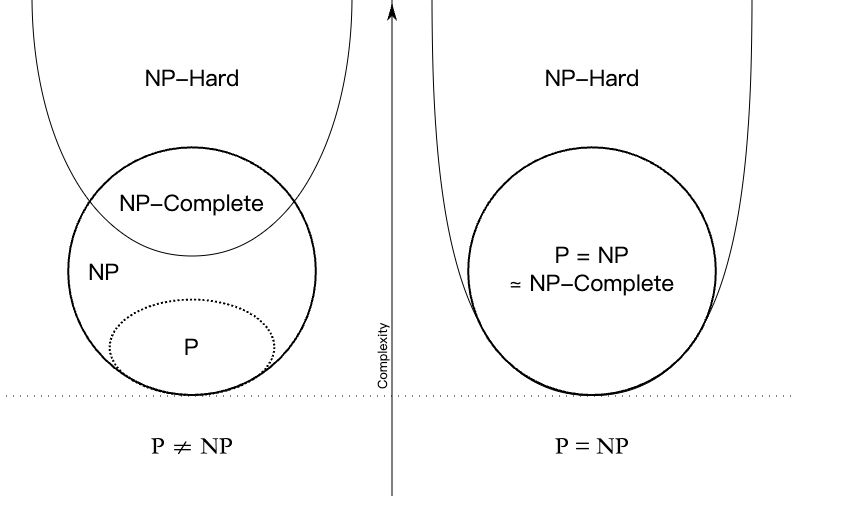
\includegraphics[width=0.6\textwidth]{./img/p_np_npc_nph.png} 
\end{figure}
\subsection{密码学基础}
参考课程\href{https://www.bilibili.com/video/BV18T411k74f/?spm_id_from=333.788&vd_source=c6586ed2410fae637f393017e00f4845}{密码学系列讲座}。
\section{区块链技术与应用}
参考课程\href{http://zhenxiao.com/blockchain/}{区块链技术与应用}。
\subsection{课程简介}

\includepdf[pages=2-6,nup=1x2]{courses/区块链技术与应用/01.pdf} 
\subsection{BTC-密码学原理}
加密货币(Crypto-currency)中主要用到密码学中的哈希函数和签名。
\subsubsection{哈希函数}
哈希函数(hash function)有两个性质:
\begin{itemize}
    \item \textbf{collision resistance (or collision free)}:不能在多项式时间内找到$x \neq y$,使得$H(x)=H(y)$。这条性质说明没有办法篡改内容而又不被检测出来。
    \item \textbf{hiding}:$x \rightarrow H(x)$是单向的,不可逆的。这里有个前提是要求输入空间大,取值分布均匀。
\end{itemize}
没有哪个哈希函数在数学上证明是collision resistance的,但是可以找到哈希碰撞的方法,例如MD5就被攻破了。

可以用哈希函数的hiding性质做digital commitment, 也就是digital equivalent of a sealed envelope。比如预测股市,先将结果放在信封里,不能提前公布预测结果,因为预测的结果可能会影响股市,接着将信封交给第三方保证不被篡改,等到开盘再打开验证。如果使用哈希函数,可以先公布哈希值$H(x)$,等到要验证时,再拿出之前写好的$x$。哈希函数hiding性质的前提是输入要足够大,分布均匀,如果输入不够大,可以在$x$后面拼接随机数$H(x||nonce)$。

bitcoin中还要求哈希函数有\textbf{puzzle friendly}性质。由于哈希值的计算事先是不可预测的,可以设置一个puzzle,比如要求计算出的哈希值前$k$个都为0,形如$00\cdots 0 $xx$\cdots$x。这其实就是挖矿,找一个随机数nonce,使得H(block header) $\le$ target,block header中含有可调节的nonce。
\begin{figure}[H]
    \centering
    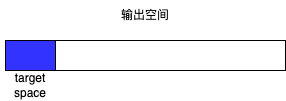
\includegraphics[width=0.4\textwidth]{courses/区块链技术与应用/lecture2/lecture1-1.png} 
\end{figure}
输出空间很大,但是目标空间很小,这只能一个一个试nonce的值。这也是工作量证明(proof of work)。虽然挖矿很难,但是验证比较容易(difficult to solve, but easy to verify)。
\subsubsection{签名}
在比特币中开户其实就是创建一个\textbf{公私钥对}(public key, private key)。公钥相当于银行账户,私钥相当于密码。在进行交易时,用私钥进行签名,说明是本人进行的,发布交易时也要发送公钥,可供他人进行验证。

在这个过程中,产生公私钥对和签名时需要一个好的随机源(a good source of randomness)。
\subsection{BTC-数据结构}
\subsubsection{哈希指针}
hash pointer
\begin{figure}[H]
    \centering
    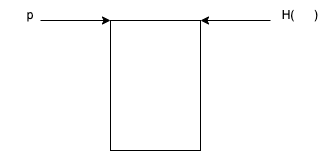
\includegraphics[width=0.4\textwidth]{courses/区块链技术与应用/lecture3/img1.png} 
\end{figure}
Block chain is a linked list using hash pointer.
\begin{figure}[H]
    \centering
    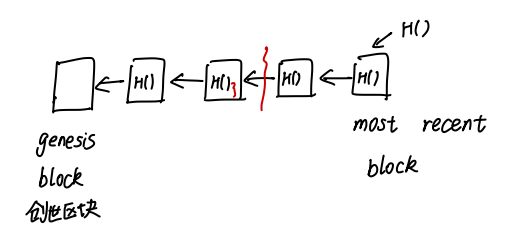
\includegraphics[width=0.5\textwidth]{courses/区块链技术与应用/lecture3/img2.png} 
\end{figure}

实现\textbf{tamper-evident log},只要保存最后一个值,就知道前面有没有修改。
\subsubsection{Merkle tree}
Merkle tree是用Hash指针代替普通指针的二叉树。
\begin{figure}[H]
    \centering
    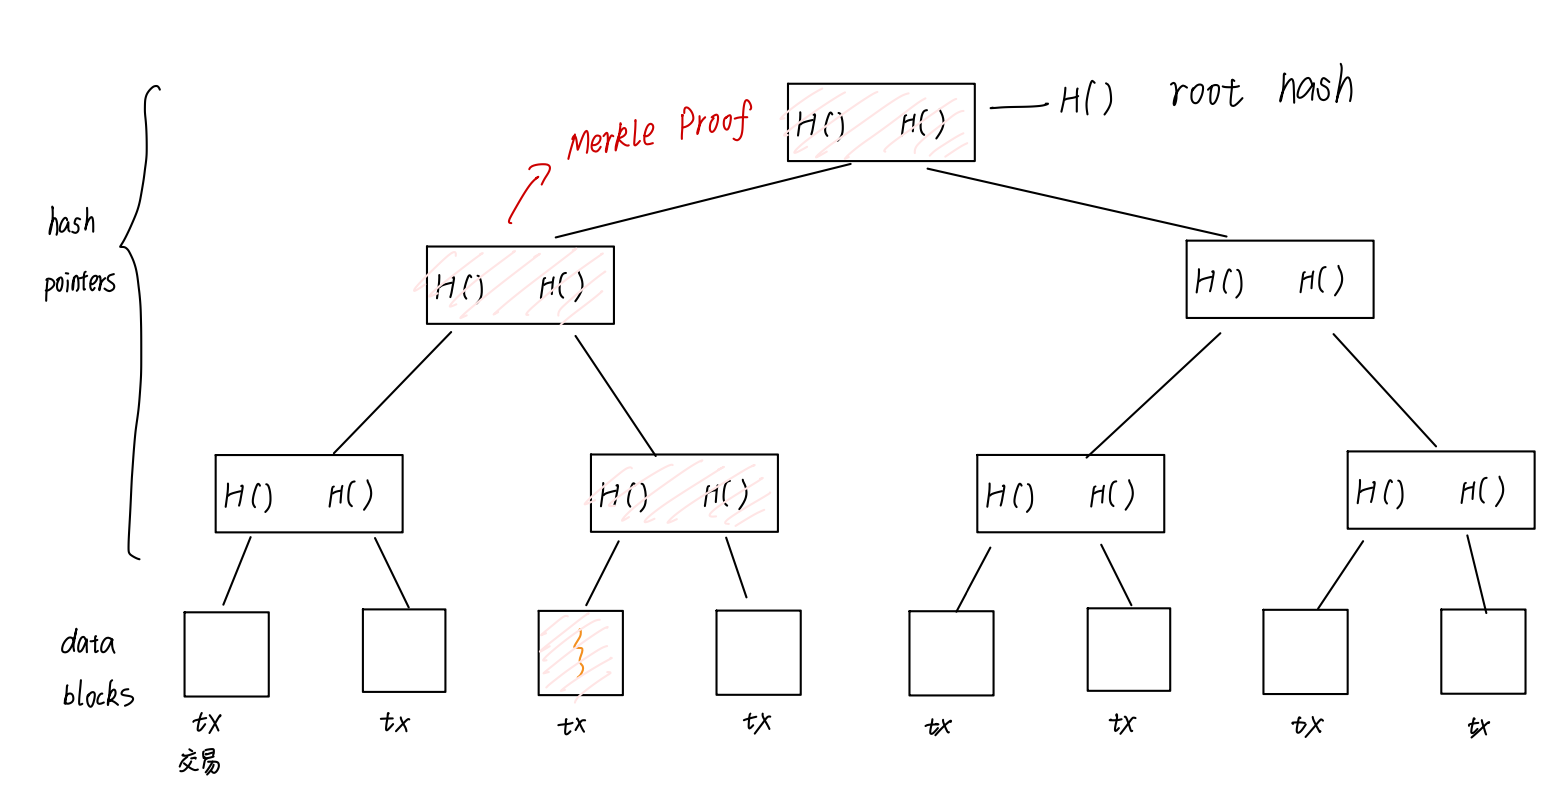
\includegraphics[width=1\textwidth]{courses/区块链技术与应用/lecture3/img3.png} 
\end{figure}
\begin{itemize}
    \item block header (有root hash)
    \item block body (有交易列表)
\end{itemize}
Merkle tree的作用是可以提供Merkle proof,证明包含某种交易(\textbf{proof of membership / proof of inclusion}),是$O(\log(n))$的时间复杂度。但是如果证明某个交易不包含在Merkle tree中,如果进行所有叶子节点的遍历,时间复杂度是$O(n)$,这时可以考虑采用sorted Merkle tree,时间复杂度降为$O(\log(n))$。
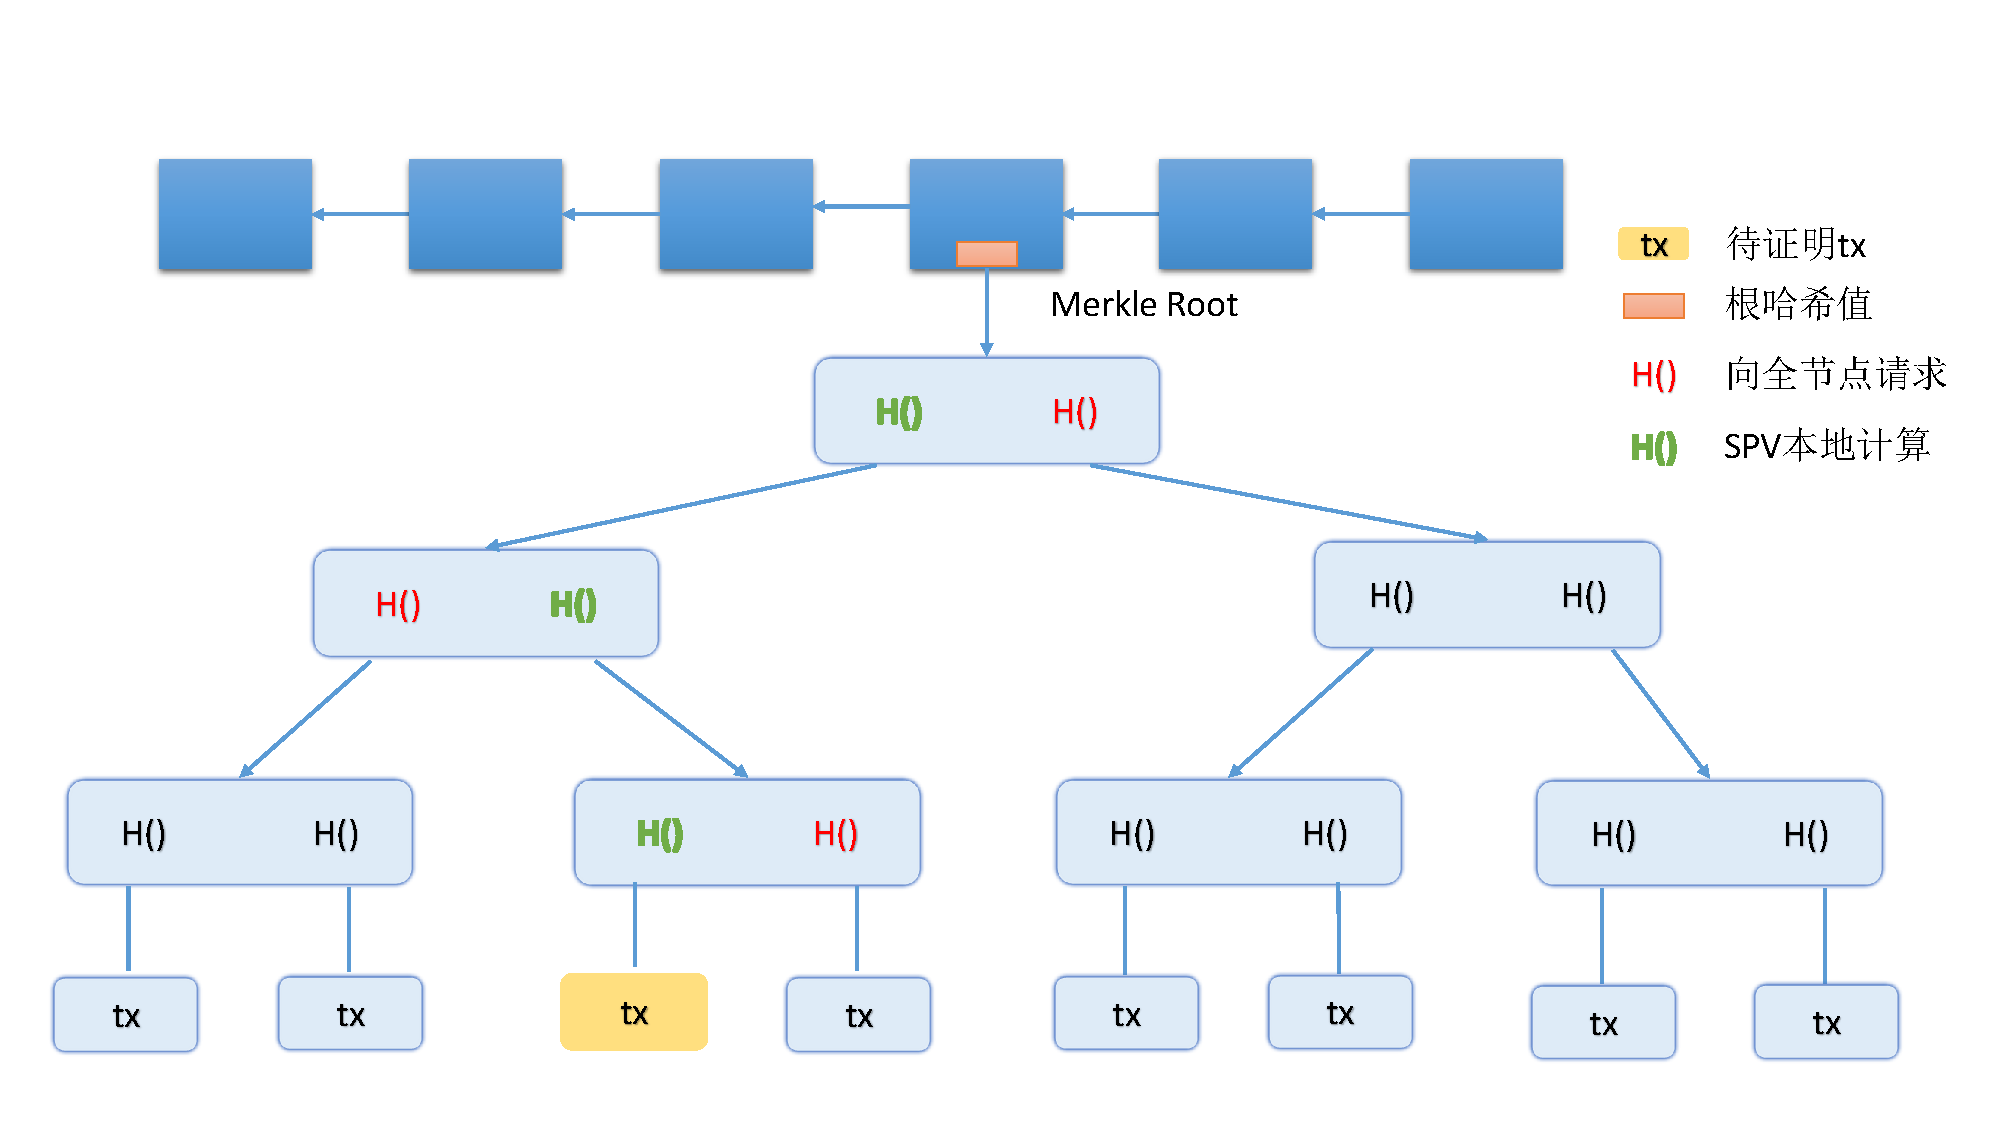
\includepdf[pages=1]{courses/区块链技术与应用/03-BTC.pdf} 
数据结构无环可以用hash pointer。如果有环会出现冲突。
\begin{figure}[H]
    \centering
    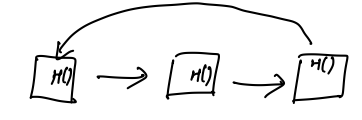
\includegraphics[width=0.5\textwidth]{courses/区块链技术与应用/lecture3/img4.png} 
\end{figure}
\subsection{BTC-协议}
如果中央银行要发售电子货币,每张纸币可以由中央银行签名。
\begin{figure}[H]
    \centering
    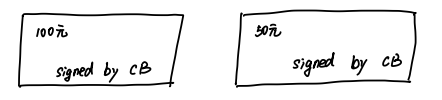
\includegraphics[width=0.5\textwidth]{courses/区块链技术与应用/lecture4/img1.png} 
\end{figure}
这会出现双花攻击(double spending attack),因为这些电子货币其实就是代码,可以进行复制,我花出去一张100的,我可以复制很多张,继续花费。可以考虑维护一个数据库,给发行的每张货币一个编号,然后记录该货币属于谁,不过这样维护数据库就很麻烦了,而且也并不是去中心化的。
\begin{figure}[H]
    \centering
    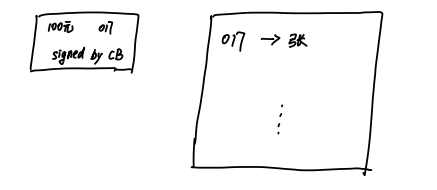
\includegraphics[width=0.5\textwidth]{courses/区块链技术与应用/lecture4/img2.png} 
\end{figure}
比特币中的交易:
\begin{figure}[H]
    \centering
    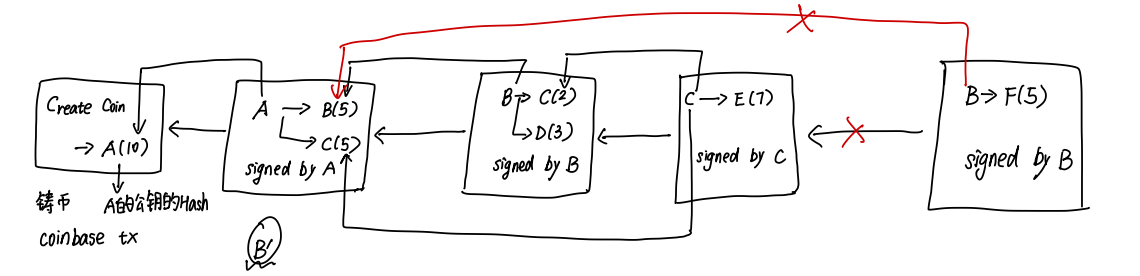
\includegraphics[width=1\textwidth]{courses/区块链技术与应用/lecture4/img3.png} 
\end{figure}
A要给B转5个比特币,A需要知道B的地址。B也需要知道A的公钥,为了验证A的签名。在上图中,在交易时不仅要说明转账的地址,也要说明币的来源。在图中第二个区块中
\begin{itemize}
    \item 输入:币的来源、A的公钥
    \item 输出:B的公钥的哈希
\end{itemize}
这里就能避免双花,例如图中最后B想给F转5个比特币,可以看到B的5个比特已经花出去了,经过检查是不能再使用的。

脚本验证(Bitcoin Script):将输入与前一个输出拼接在一起,看是否能正确运行。
\begin{figure}[H]
    \centering
    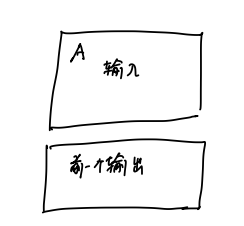
\includegraphics[width=0.3\textwidth]{courses/区块链技术与应用/lecture4/img4.png} 
\end{figure}
每个块可以有很多交易,组织成Merkle tree。
\begin{figure}[H]
    \centering
    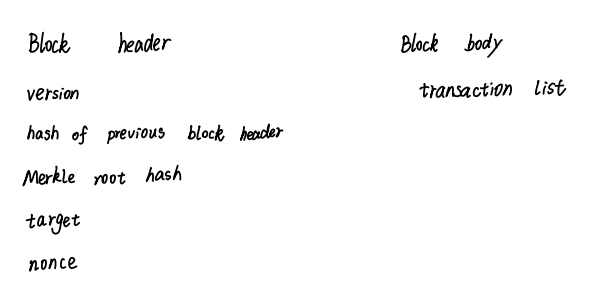
\includegraphics[width=0.7\textwidth]{courses/区块链技术与应用/lecture4/img5.png} 
\end{figure}
\textbf{挖矿}:H(block header)$\le$target.区块链的另一种画法,因为其实哈希指针计算的是前一个block header中的哈希。
\begin{figure}[H]
    \centering
    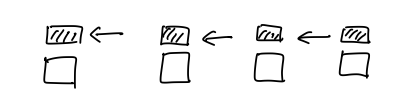
\includegraphics[width=0.6\textwidth]{courses/区块链技术与应用/lecture4/img6.png} 
\end{figure}
\begin{itemize}
    \item full node: fully validating node,全节点记录所有信息
    \item light node: 轻节点
\end{itemize}

账本的内容要取得分布式的共识(distrubted consensus)。

FLP impossibilty result: 在异步系统中,网络传输时延没有上限,哪怕系统中只有一个成员是faulty,也没法达成共识。

CAP Theorem:任何一个分布式系统,以下3个性质中最多满足2个。
\begin{itemize}
    \item C: Consistency 一致性
    \item A: Availability
    \item P: Partition tolerance
\end{itemize}
Paxos协议满足Consistency性质。
\subsubsection{Consensus in BitCoin}
重要的问题是:成员(membership)中谁拥有投票权。联盟链(hyperledger fabric)是只有加入链的成员有投票权。

女巫攻击(sybil attack):攻击方产生超过一半的用户。

如果节点能解决puzzle问题,可以获得记账权,有权利发布下一个节点。
\begin{figure}[H]
    \centering
    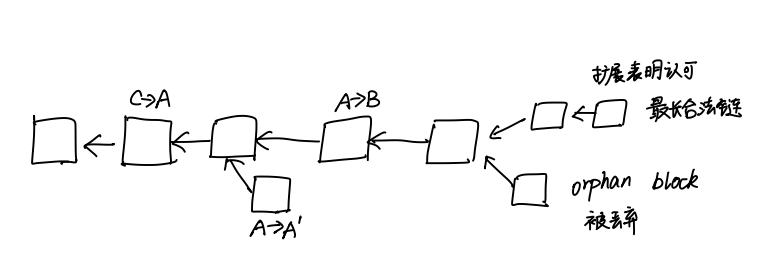
\includegraphics[width=1\textwidth]{courses/区块链技术与应用/lecture4/img7.png} 
\end{figure}
longest vaild chain: 最长合法链

forking attack: 分叉攻击

block reward: 出块奖励

mining: 挖矿

miner: 矿工

coinbase transaction 是产生币的唯一方法。每隔21万个区块,区块奖励减半,50BTC$\rightarrow$25BTC$\rightarrow$12.5BTC.
\subsection{BTC-实现}
比特币是基于交易记录的模式(\textbf{transaction-based ledger})。

\textbf{UTXO}: Unspent Transaction Output 还未花掉的交易的输出,为了检测双花,包含产生交易的哈希值以及在交易中的第几个。
\begin{figure}[H]
    \centering
    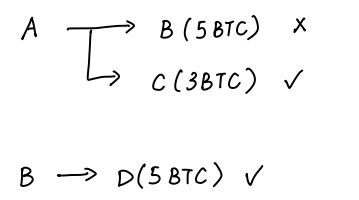
\includegraphics[width=0.4\textwidth]{courses/区块链技术与应用/lecture5/img1.png} 
\end{figure}
B的5BTC已经花出去了,因此不在UTXO中。

total inputs = total outputs 所有输入=所有输出,但有时候不完全相等,例如所有输入为1BTC,所有输出为0.99BTC,这其中的差值是交易费(transaction fee)。比特币中大约每4年区块奖励会减半,因此到后期的奖励可能大部分来自于交易费。
$$
\frac{\text{21万区块}\times\text{10分钟}}{\text{60分钟}\times\text{24小时}\times\text{365天}} \approx \text{4年}
$$
还有一种模式是基于账户的模式(\textbf{account-based ledger}),例如以太坊。
\begin{figure}[H]
    \centering
    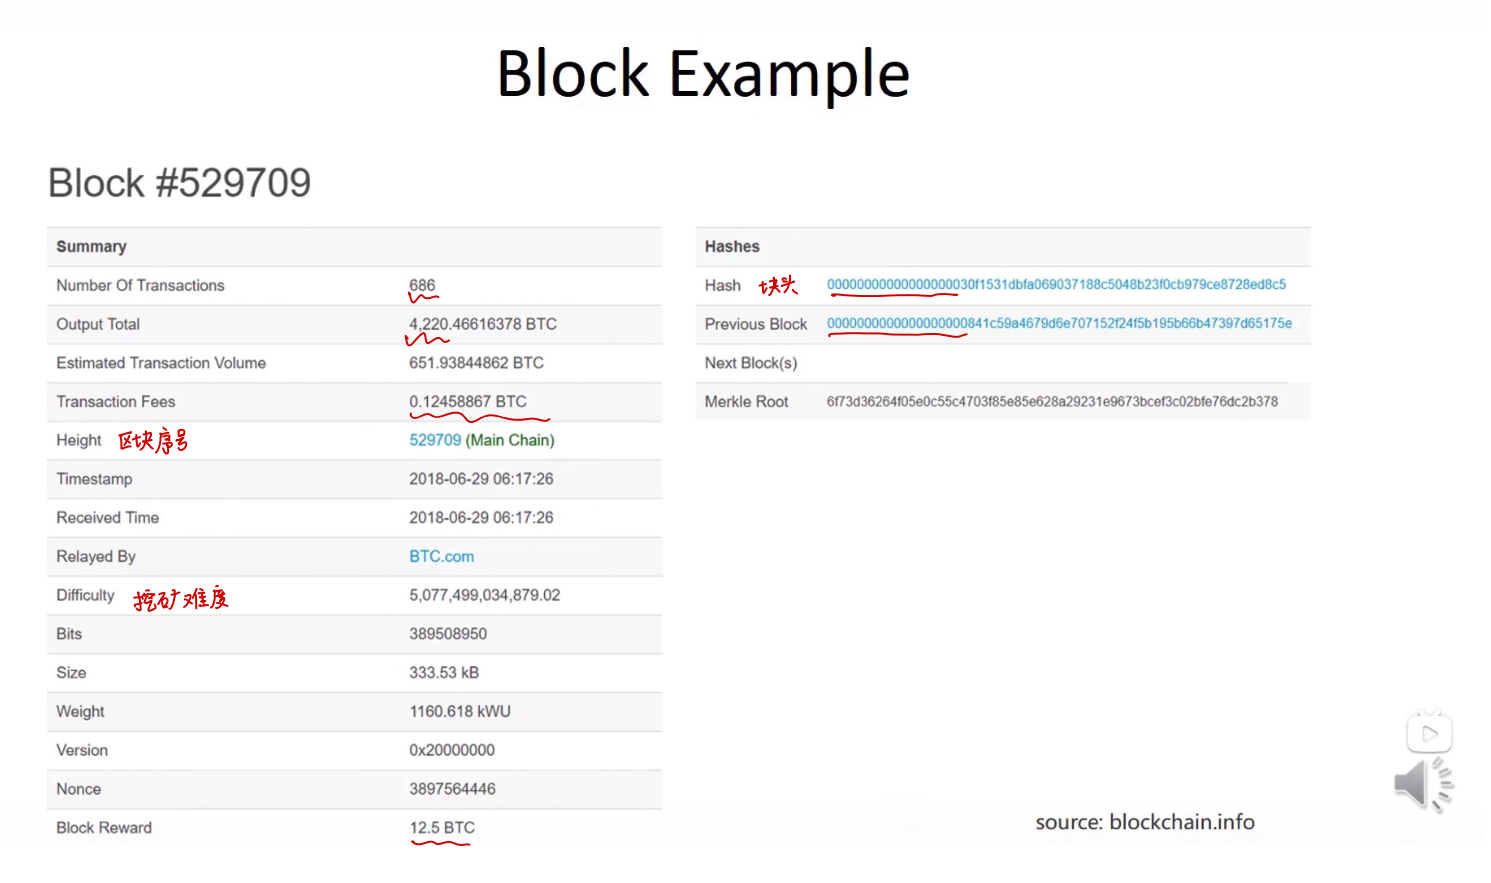
\includegraphics[width=1\textwidth]{courses/区块链技术与应用/lecture5/img2.png} 
\end{figure}
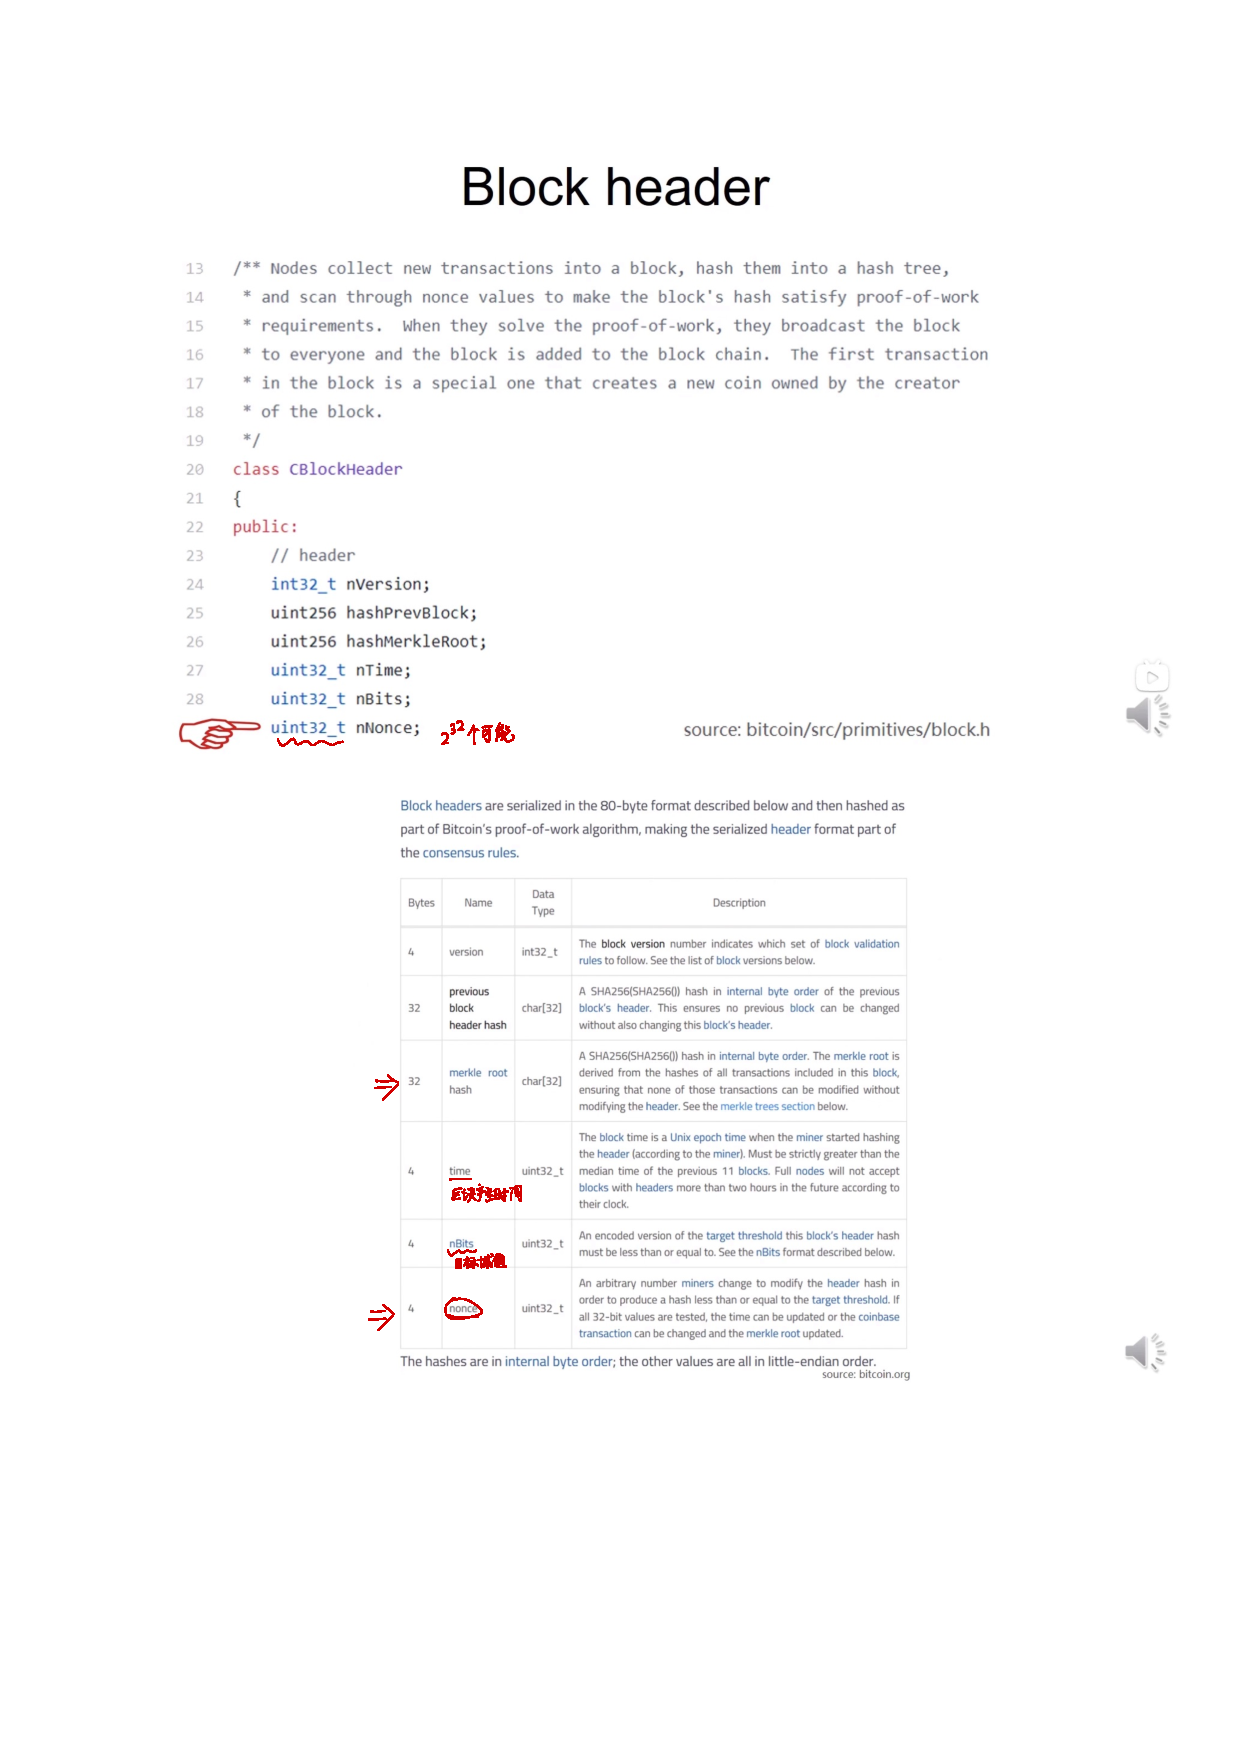
\includepdf[pages=-]{courses/区块链技术与应用/lecture5/1.pdf} 
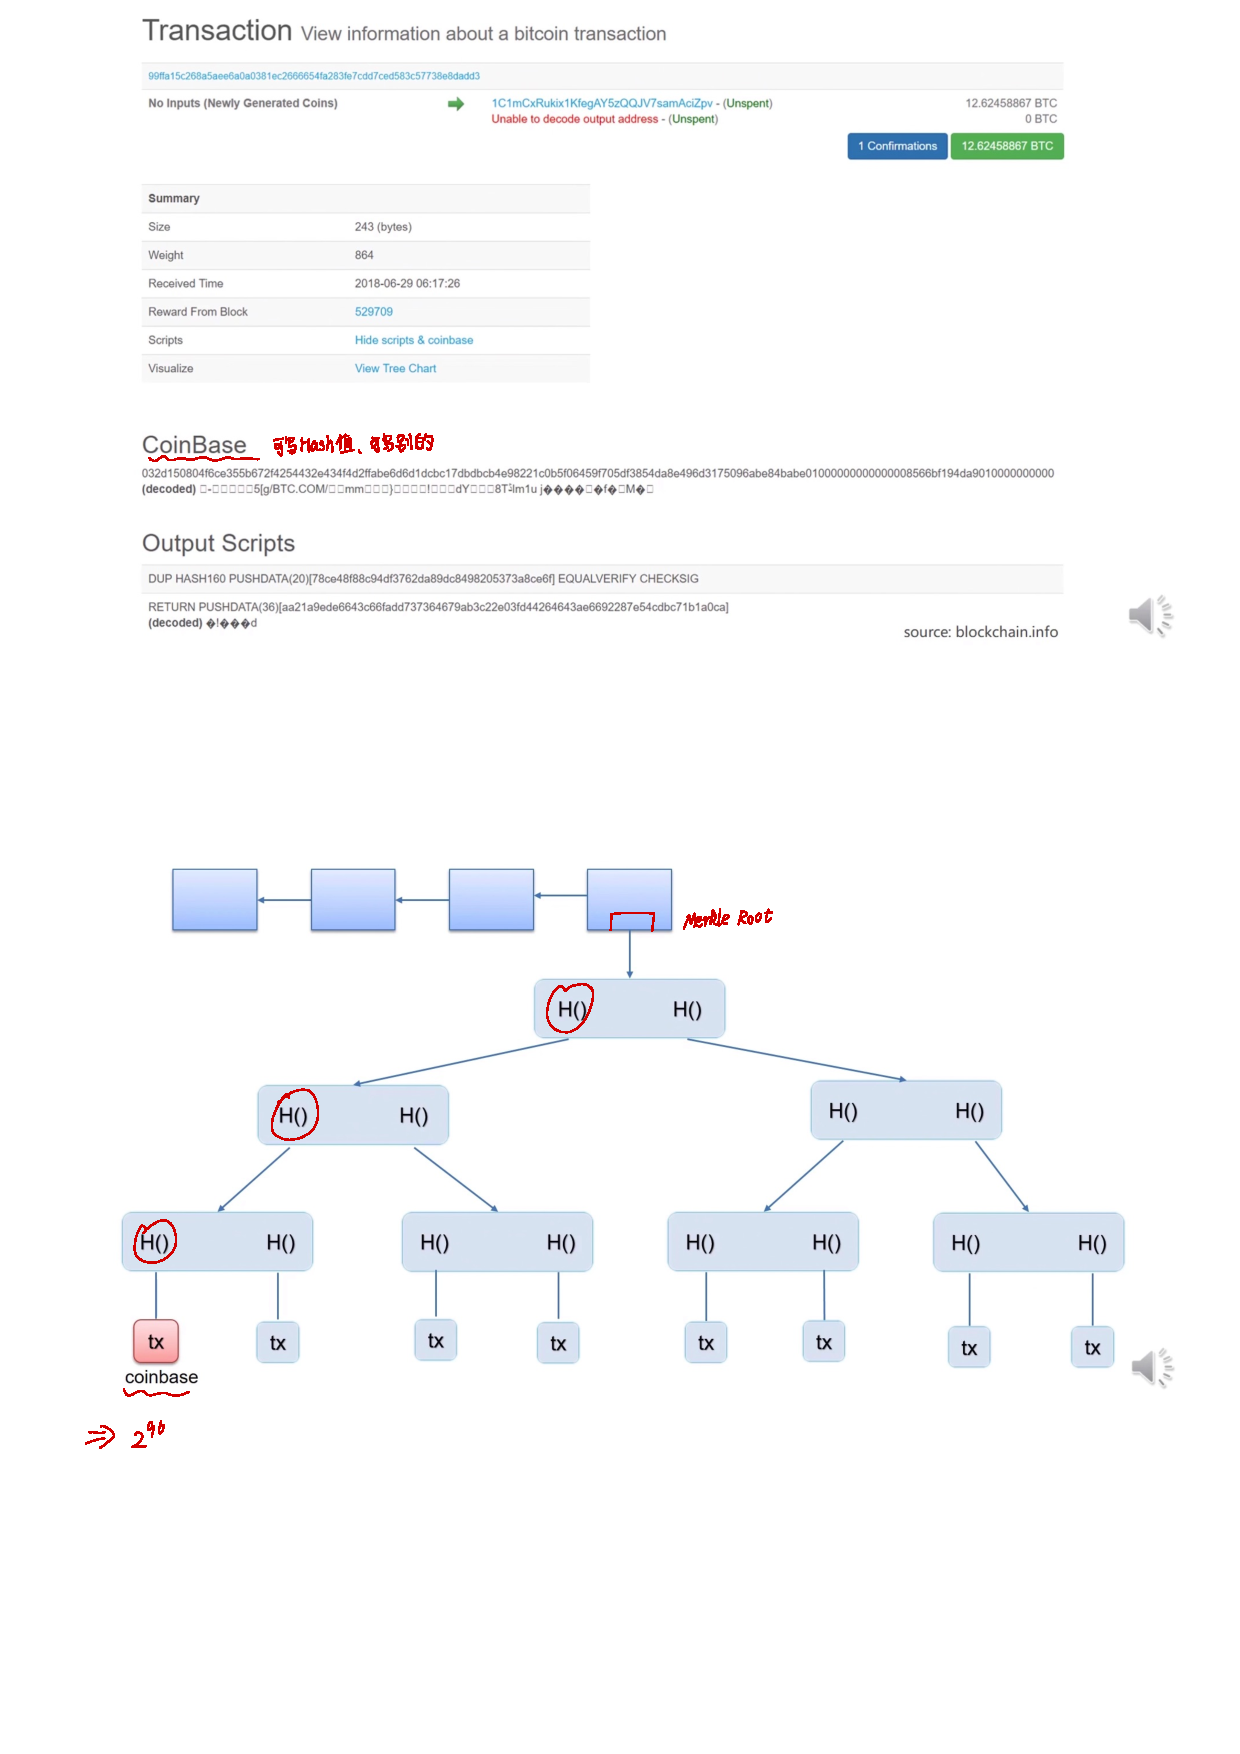
\includepdf[pages=-]{courses/区块链技术与应用/lecture5/2.pdf} 
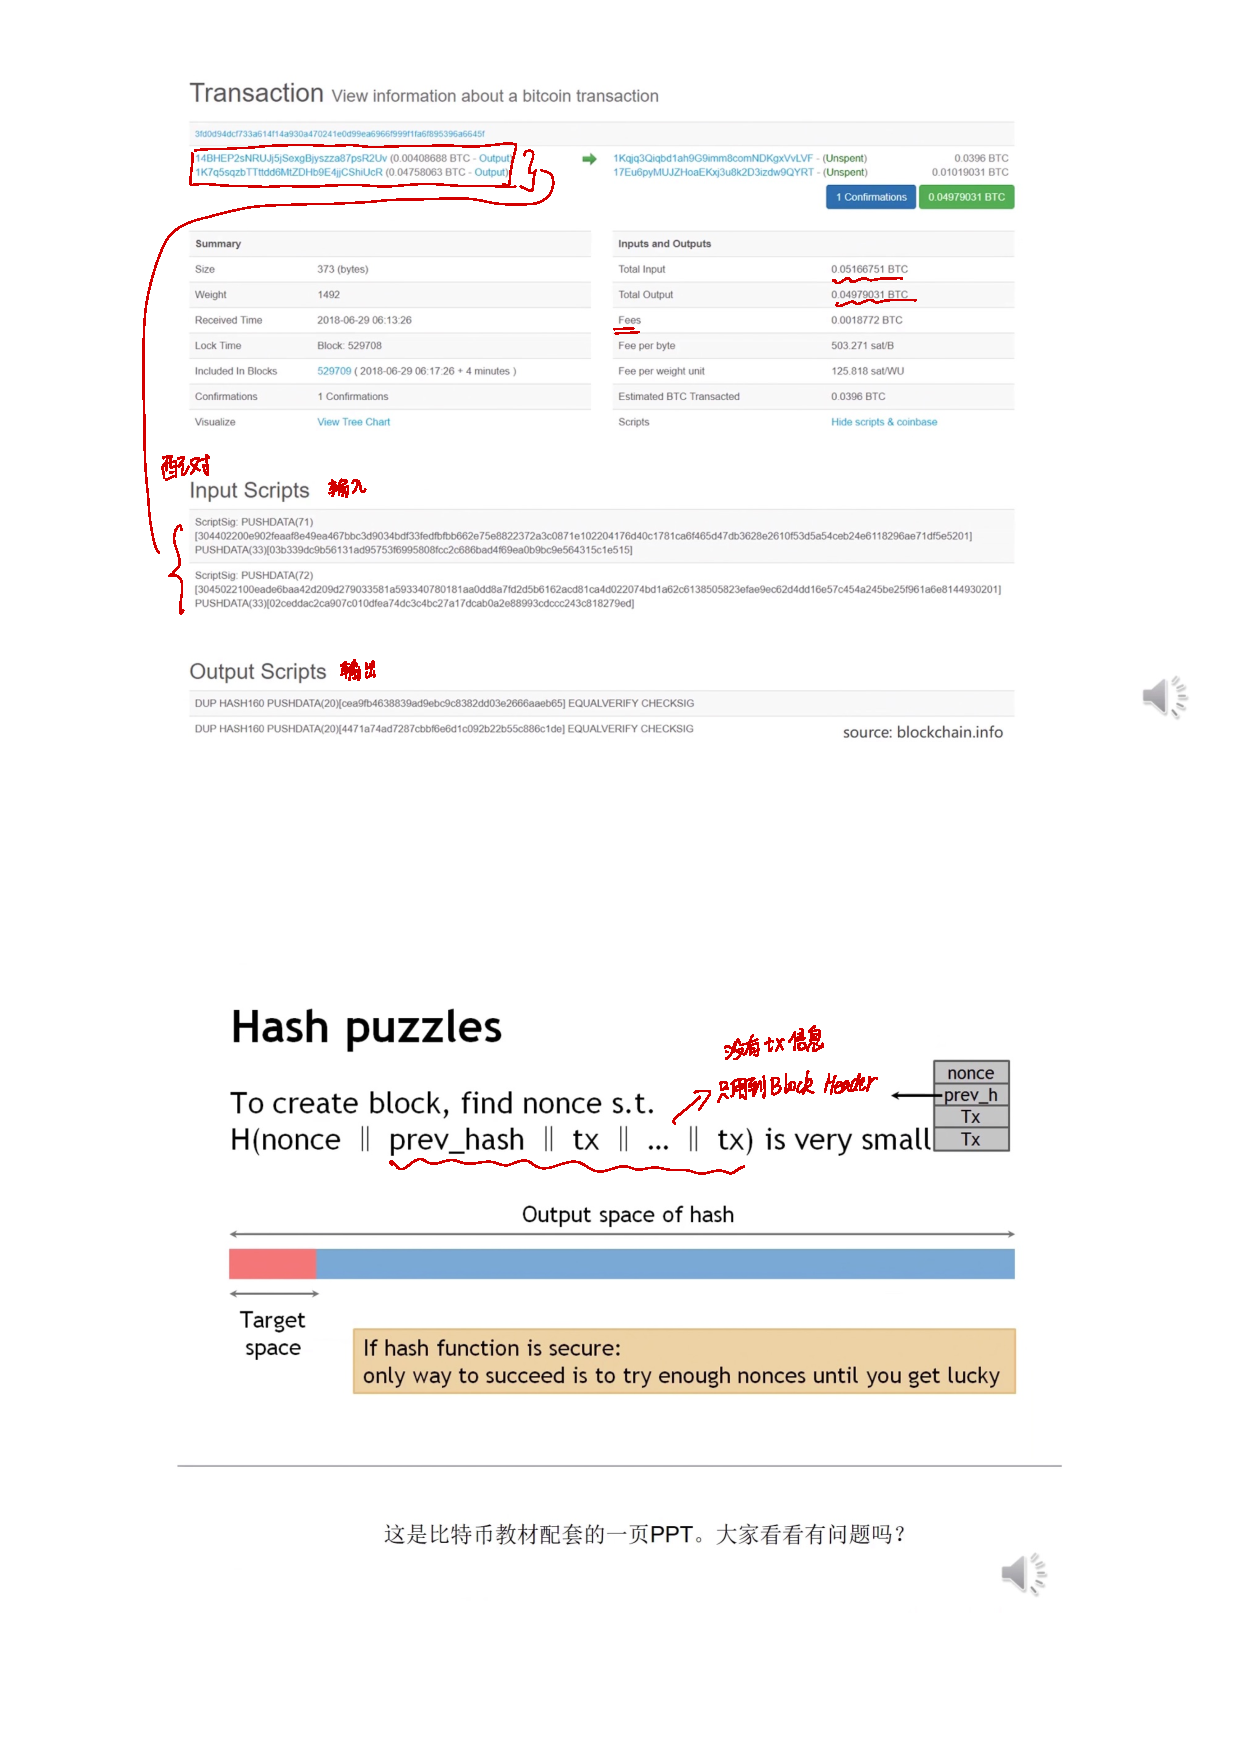
\includepdf[pages=-]{courses/区块链技术与应用/lecture5/3.pdf} 
每次挖矿尝试看作是\textbf{Bernoulli trial}: a random experiment with binary outcome. Bernoulli process: a sequence of independent Bernoulli trials. Bernoulli process具有无记忆性(\textbf{memoryless})。大量的Bernolli process可用Poisson process近似。

出块时间服从指数分布(exponential distrubtion),也具有无记忆性。
\begin{figure}[H]
    \centering
    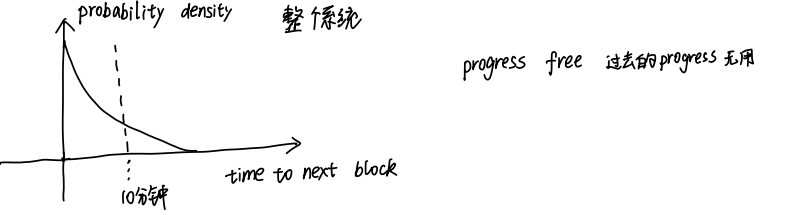
\includegraphics[width=1\textwidth]{courses/区块链技术与应用/lecture5/img3.png} 
\end{figure}
产生比特币数量构成几何序列(geometric series)
\begin{figure}[H]
    \centering
    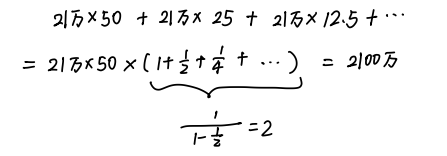
\includegraphics[width=0.5\textwidth]{courses/区块链技术与应用/lecture5/img4.png} 
\end{figure}
BitCoin is secured by mining.
\begin{figure}[H]
    \centering
    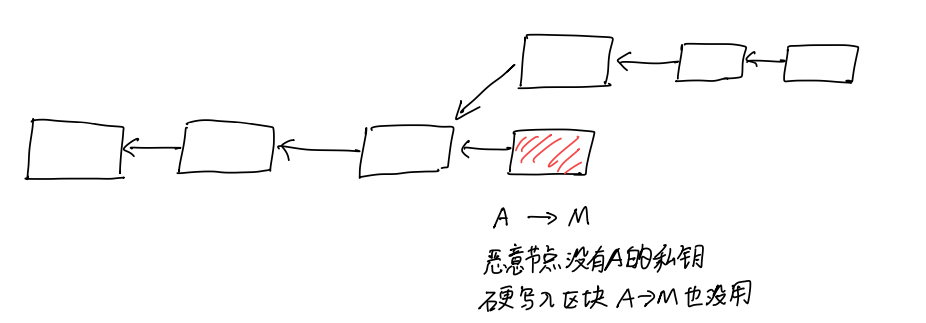
\includegraphics[width=1\textwidth]{courses/区块链技术与应用/lecture5/img5.png} 
\end{figure}
double spending
\begin{figure}[H]
    \centering
    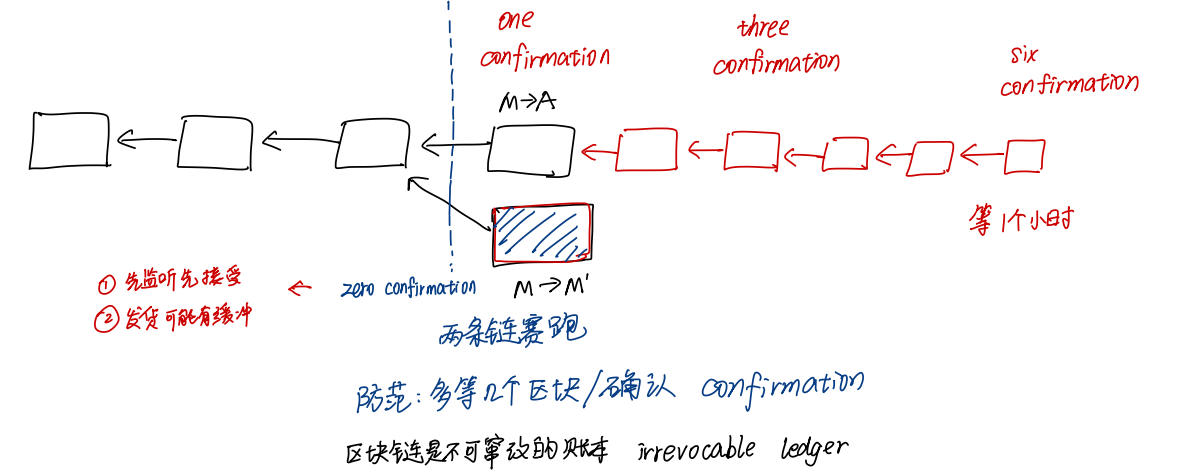
\includegraphics[width=1\textwidth]{courses/区块链技术与应用/lecture5/img6.png} 
\end{figure}
selfish mining的分叉攻击,挖一长串,然后一下发布,这么做是有风险的。
\begin{figure}[H]
    \centering
    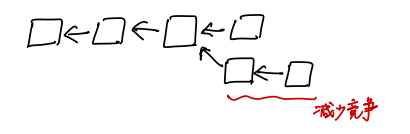
\includegraphics[width=0.5\textwidth]{courses/区块链技术与应用/lecture5/img7.png} 
\end{figure}
\subsection{BTC-网络}
上层是application layer: BitCoin Block chain.下层是network layer: P2P Overlay Network.比特币中各节点是对等的。

比特币网络设计原则:simple, robust(鲁棒), but not efficient.

flooding, 邻居节点的选取是随机的,因此两个节点可能地理上相隔很远,网络传输慢,并不是非常有效。全节点维护一个等待上链的集合,第一次听到转发,会在该集合中删除该交易,后续不转发。区块大小限制在1M。网络传播是尽力交付(best effort)。

\subsection{BTC-挖矿难度}
H(block header) $\le$ target,挖矿难度
$$
\text{difficulty} = \frac{\text{difficulty\_1\_target}}{\text{target}}
$$
难度1,target更大。挖矿难度与target成反比。
\begin{figure}[H]
    \centering
    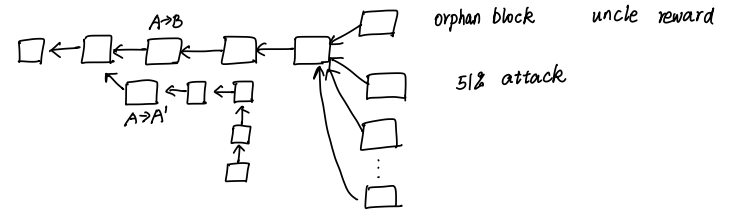
\includegraphics[width=1\textwidth]{courses/区块链技术与应用/lecture7/img1.png} 
\end{figure}
出块时间越短,出现分叉的可能更多。

以太坊协议 ghost,平均出块时间需要保持稳定。

调整挖矿难度:
$$
\text{target} = \text{target} \times \frac{\text{actual time}}{\text{expected time}}
$$
其中,acutual time是最近挖出2016区块的时间,期望时间expected time = $2016 \times 10$,理想的挖出2016个区块的时间是两周。难度最大增长4倍,最小也是缩小4倍。
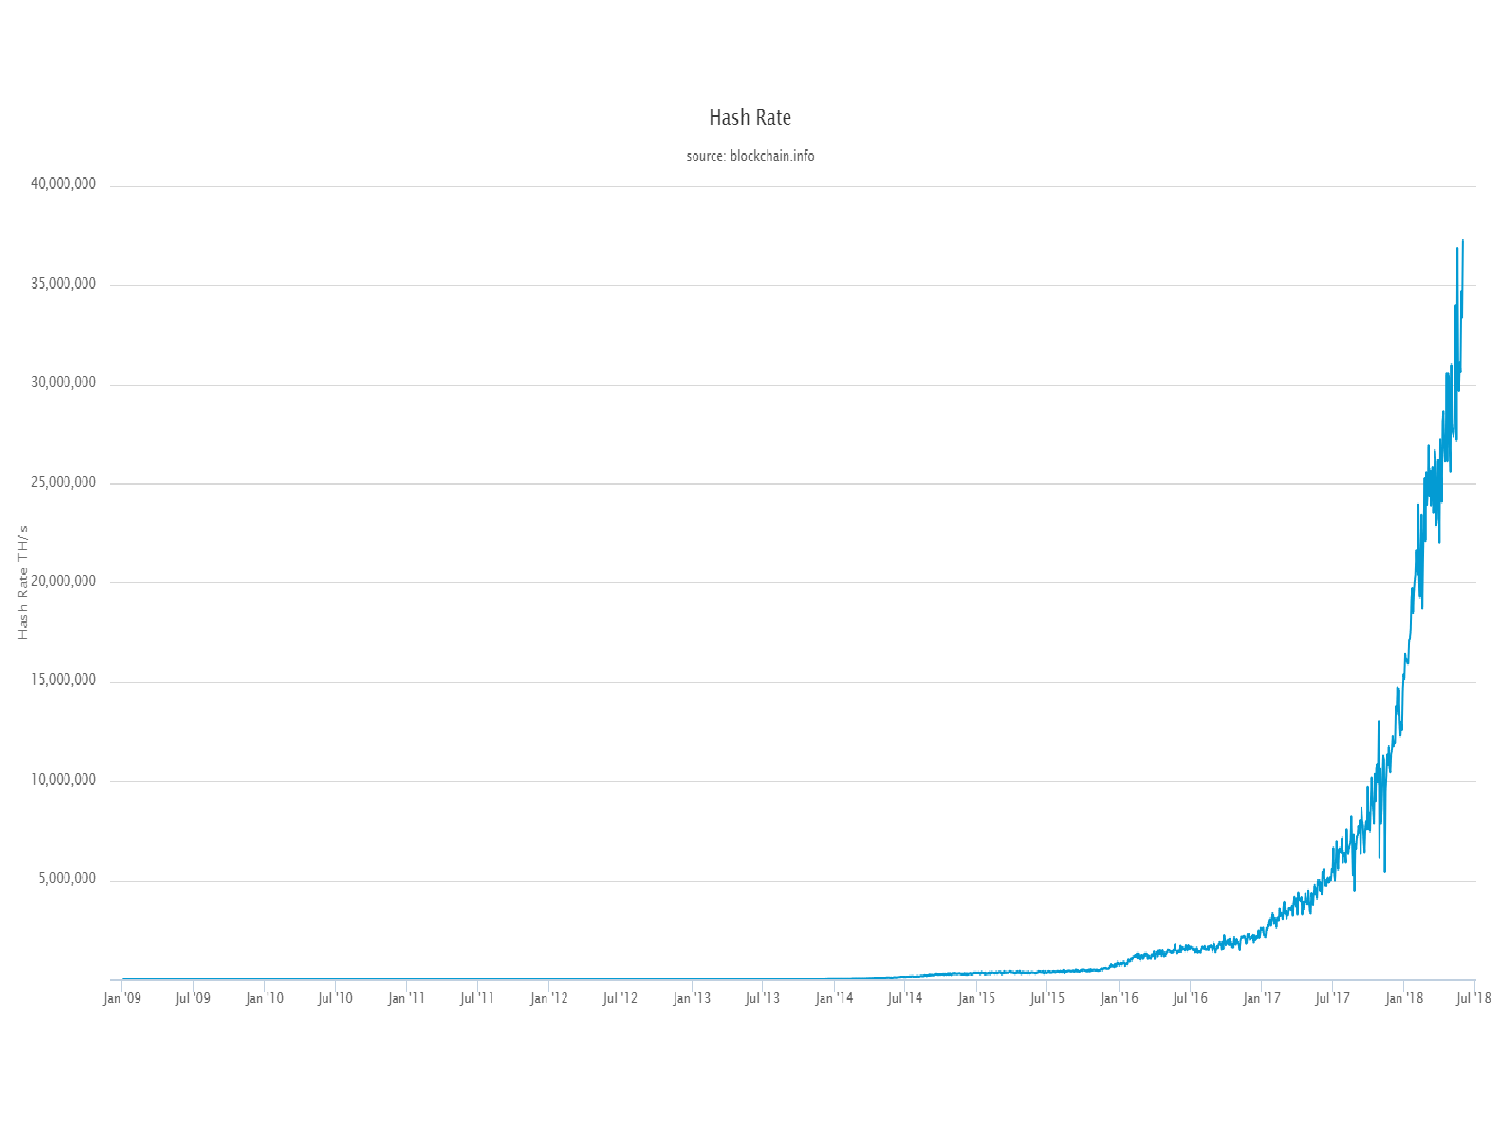
\includepdf[pages=-,nup=1x2]{courses/区块链技术与应用/07-BTC.pdf} 
\subsection{BTC-挖矿}
全节点验证合法性包括:每个交易合法、发布区块难度以及延伸最长合法链。

挖矿无记忆性,memoryless以及progress free。

比特币安全性由密码学安全与共识机制保证,这个前提是大部分节点是好的节点。

CPU$\rightarrow$ GPU挖矿$\rightarrow$ ASIC(Application Specific Integrated Circuit)芯片,ASIC芯片只能挖同一个mining puzzle的货币。有的币设计之初选择Alternative mining puzzle,设计出发点是ASIC resistance。

矿池,一个矿主(pool manager)下面有许多矿工(miner),矿主承担全节点其他功能。矿池的出现解决矿工收入不稳定的问题。通过工作量证明来分配收入,例如本来要求nonce使得前面60个为0,降低难度,如果求出该问题的nonce,则获得一个share,将almost vaild block提交给矿主,证明工作,最后根据提交的share数量分配奖励。

转换矿池很容易,大型矿池如果有51\%算力,可发起攻击:
\begin{itemize}
    \item 分叉攻击
    \begin{figure}[H]
        \centering
        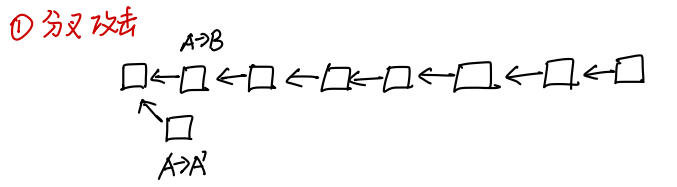
\includegraphics[width=0.7\textwidth]{courses/区块链技术与应用/lecture8/img1.png} 
    \end{figure}
    \item Boycott 封锁,和A有关交易都不包含,马上分叉
    \begin{figure}[H]
        \centering
        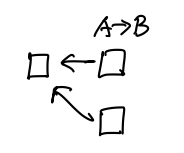
\includegraphics[width=0.2\textwidth]{courses/区块链技术与应用/lecture8/img2.png} 
    \end{figure}
\end{itemize}
但是拥有51\%以上算力不能盗币,因为没有别人账户的私钥。如果强行发布不合法的区块,会造成分叉。

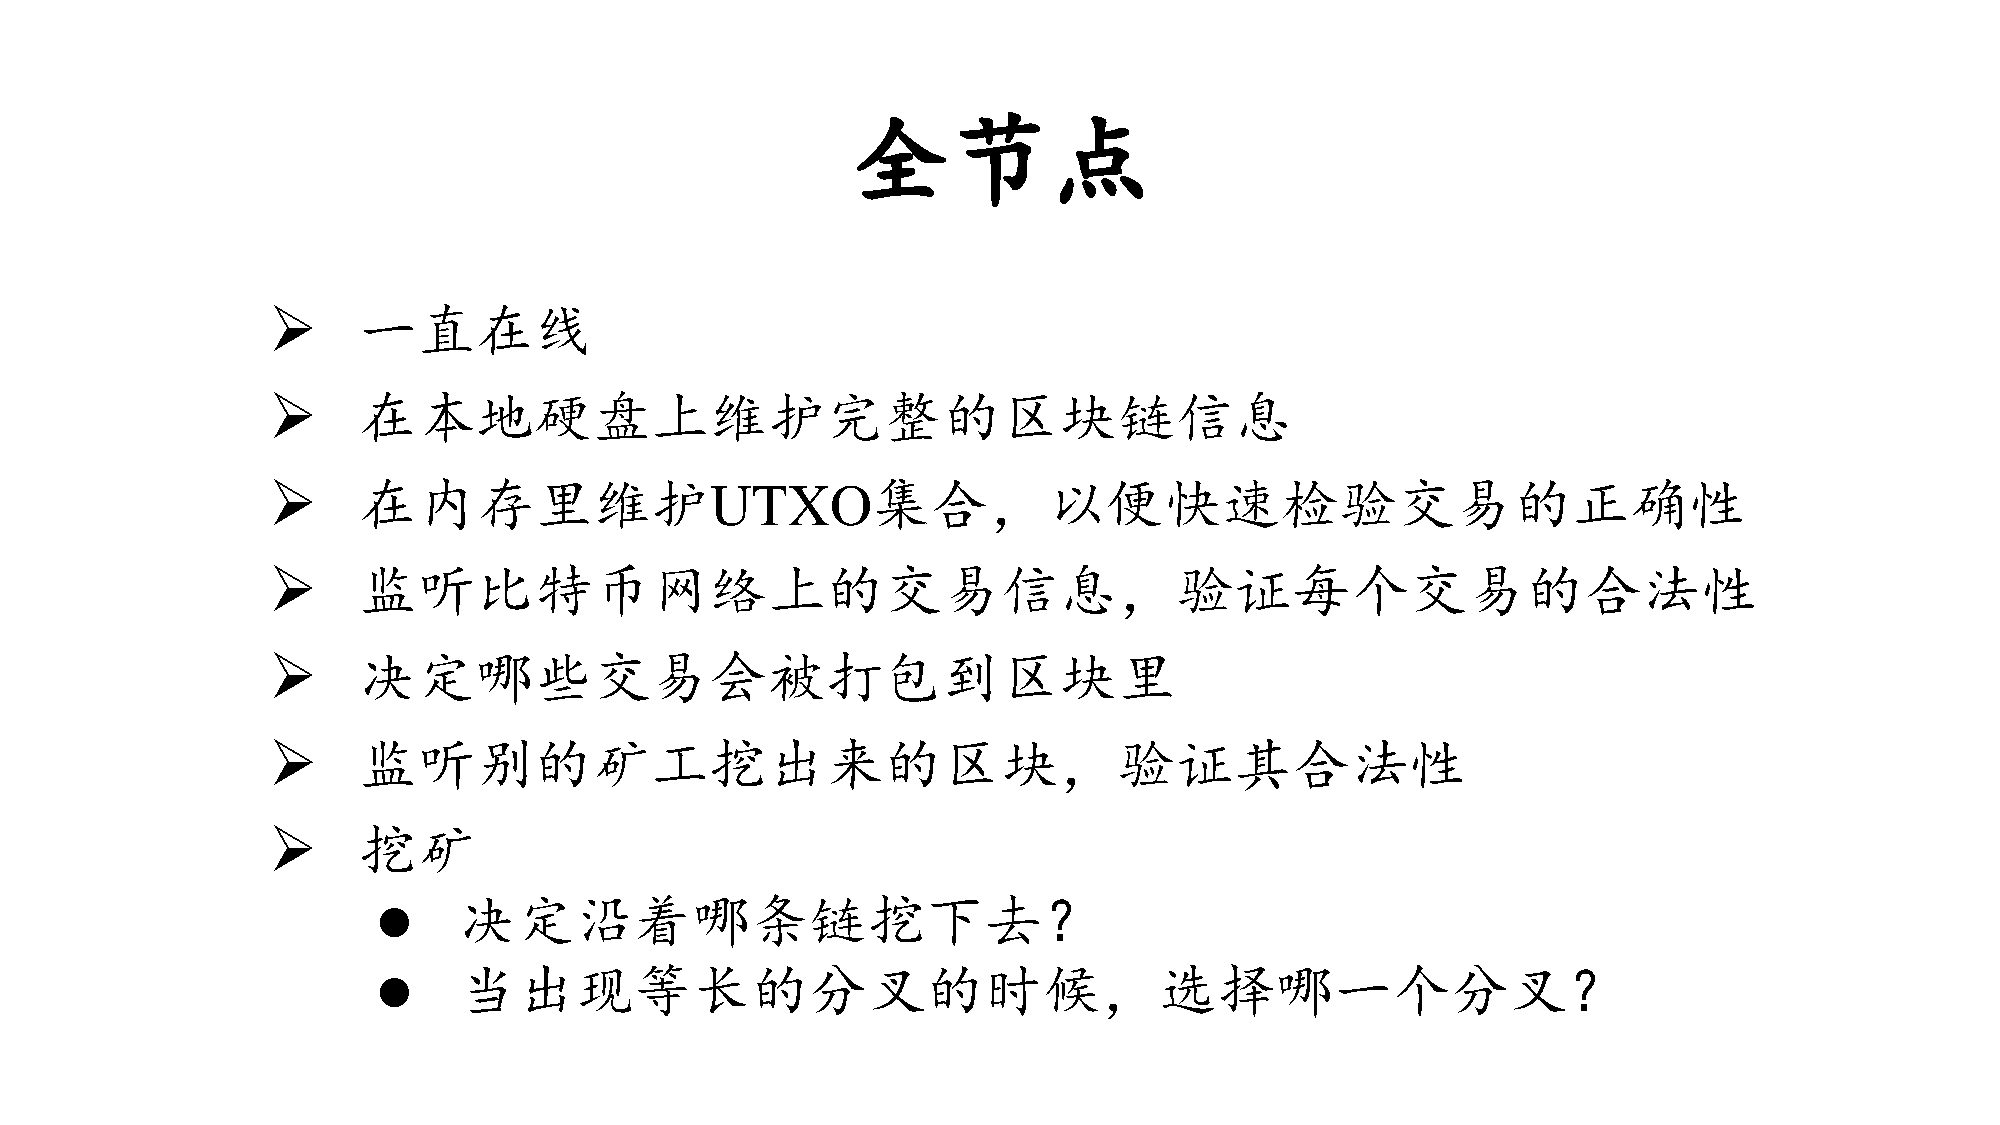
\includepdf[pages=-,nup=1x2]{courses/区块链技术与应用/08-BTC.pdf}  
\subsection{BTC-比特币脚本}
交易结构:
\begin{itemize}
    \item version: 比特币协议版本号
    \item locktime: 生效时间
    \item blockhash: 交易所在区块的hash值
    \item blocktime: 区块产生时间
\end{itemize}
交易的输入:
\begin{itemize}
    \item "txid"与"vout",表示币的来源
    \item "scriptSig"表示输入脚本
\end{itemize}
交易的输出:
\begin{itemize}
    \item "value":输出金额
    \item "n":序号
    \item "scriptPubKey": 输出脚本
    \item "reqSigs":需要多少个签名
    \item "type": 输出类型
\end{itemize}
redeemScript: 赎回脚本

多重签名:
\begin{itemize}
    \item 多重签名要求N个人中有M个签名
    \item x是代码实现的bug,往栈里多压入一个元素
    \item 输入脚本中M个签名的顺序要与输出脚本中的pubkey相同
\end{itemize}

用P2SH实现多重签名的好处是在用户端,也就是输出脚本处,只需要得知赎回脚本的哈希值即可,不需要N个公钥。同时赎回脚本中方便修改N与M的值。

Proof of Burn
\begin{itemize}
    \item RETURN: 无条件返回错误,可用于证明销毁比特币
    \item 可以往区块链中写入内容,digital commitment,比如用作知识产权。还有另一个域coinbase域,可以往区块链中写入内容。
\end{itemize}

在实际中,操作中含有前缀,例如OP\_CHECKSIG、OP\_DUP,课程中做了简化。

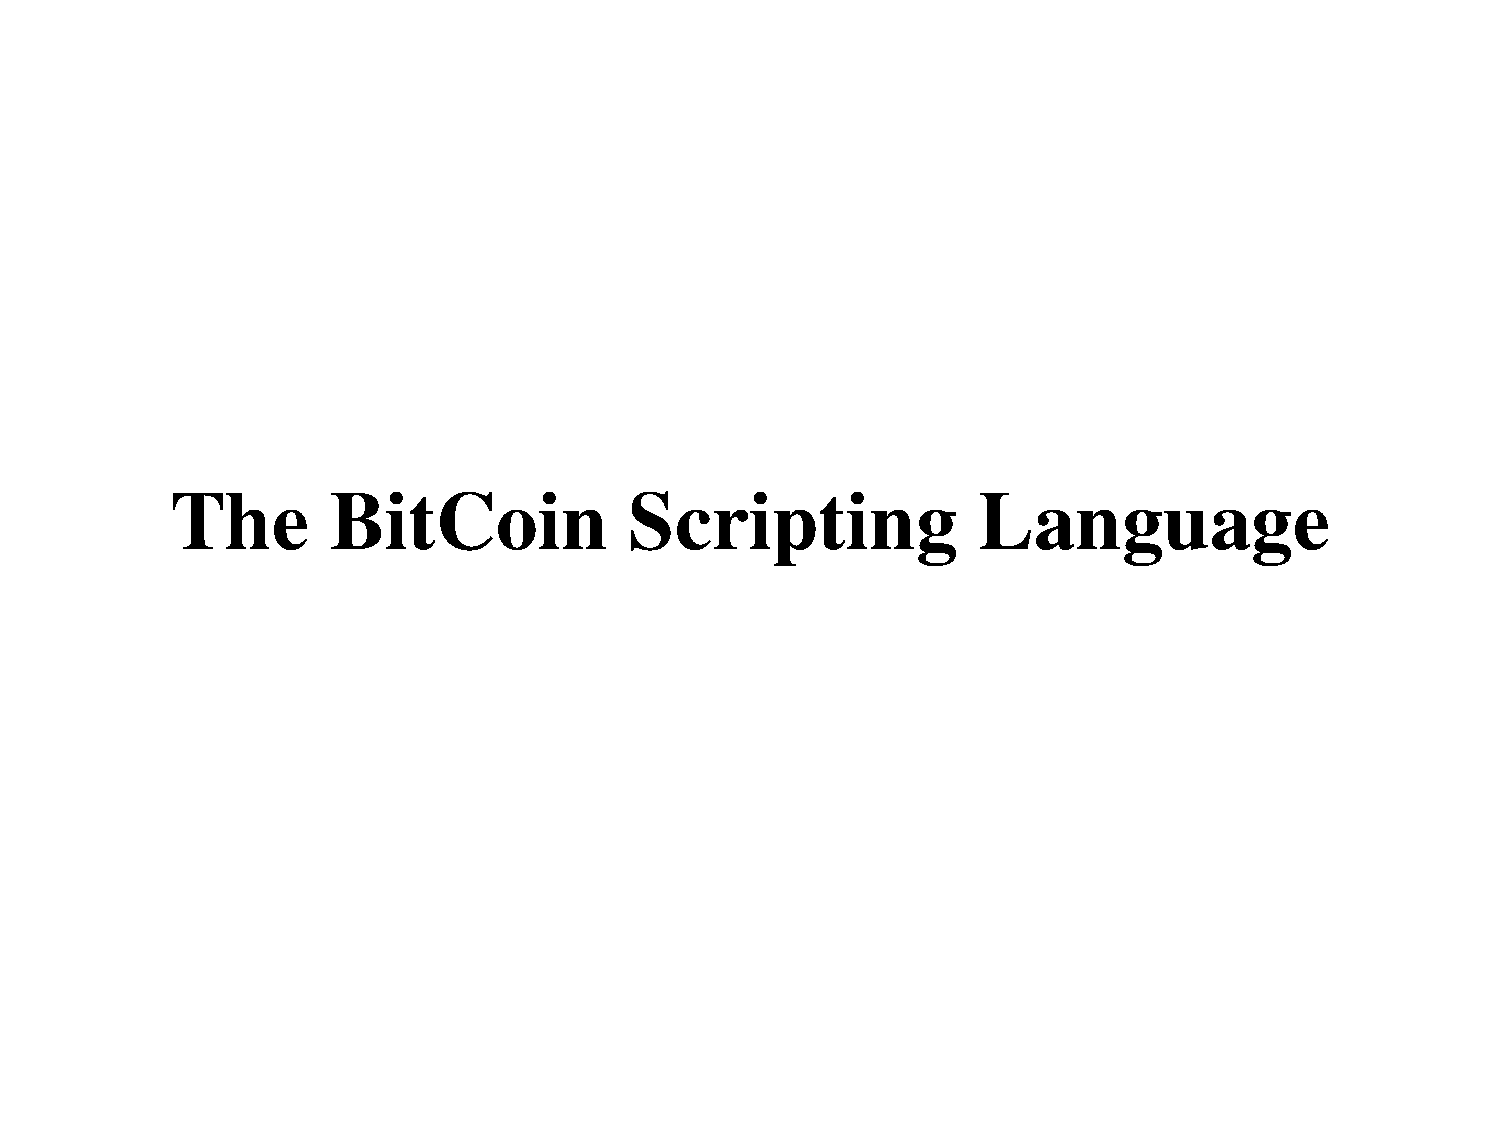
\includepdf[pages=-,nup=1x2]{courses/区块链技术与应用/09-BTC.pdf}  
\subsection{BTC-分叉}
\begin{itemize}
    \item state fork:当前状态产生分歧,例如分叉攻击(forking attack),也叫做deliberate fork。
    \item protocol fork:对协议产生分歧
\end{itemize}
还有一种分类是分为硬分叉和软分叉。
\subsubsection{hard fork}
例如block size limit的改变,原来为1M,当block size limit为1M时,一个交易大约是250个字节,一个block可以产生1000,000/250 = 4000个交易,而一个block产生需要10分钟,因此每秒产生4000/(60 $\times$ 10) $\approx $7个交易。这个交易产生的数量太少,并且会有延迟,一个交易可能这个区块没写进去,会等到下一个区块,这就要等待10分钟。考虑block size limit从1M $\rightarrow$ 4M。
\begin{figure}[H]
    \centering
    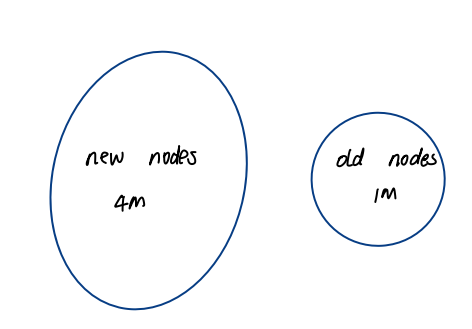
\includegraphics[width=0.6\textwidth]{courses/区块链技术与应用/lecture10/img1.png} 
\end{figure}
如上图所示,拥有大多数算力节点承认区块大小限制为4M,旧节点承认区块大小为1M。
\begin{figure}[H]
    \centering
    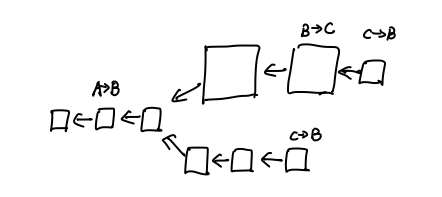
\includegraphics[width=0.6\textwidth]{courses/区块链技术与应用/lecture10/img2.png} 
\end{figure}
这样会造成永久性分叉,旧节点不承认新节点,会按照原来的链挖,而新节点也是承认1M区块大小的。如果出现下面的链进行交易回放,如C$\rightarrow$B,可以加上chainID来解决这个问题。
\subsubsection{soft fork}
比特币协议中加一些限制,使得原来合法的交易变得不合法,造成了软分叉。例如区块的大小限制1M变为0.5M。
\begin{figure}[H]
    \centering
    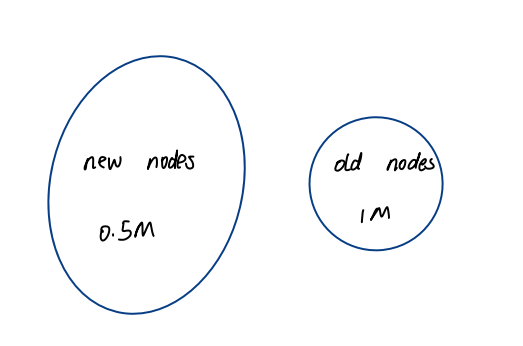
\includegraphics[width=0.6\textwidth]{courses/区块链技术与应用/lecture10/img3.png} 
\end{figure}
软分叉是临时的,旧节点也认可新节点的链,旧节点会在最长合法链后面挖,不然自己就白挖了。
\begin{figure}[H]
    \centering
    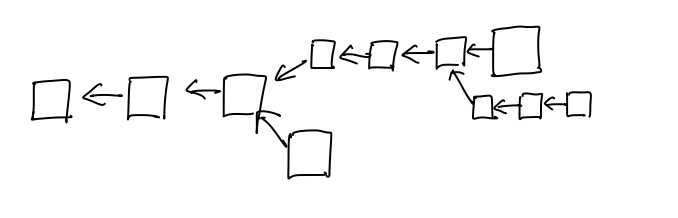
\includegraphics[width=0.6\textwidth]{courses/区块链技术与应用/lecture10/img4.png} 
\end{figure}
现实中的软分叉:给目前域赋予新的含义,例如coinbase域。原来调整extra nonce,有4bytes,搜索空间是$2^{32}$,可以加上coinbase的前8bytes,搜索空间变为$2^{96}$。

我们知道Merkle proof可以证明某个交易是否在区块里,但是如果想证明某个账户A上有多少钱,全节点可以查看账户A在UTXO对应的输出,对于区块链钱包,也就是轻节点,可以向全节点发出一个请求,全节点返回一个结果,但无法证明该结果是否正确。解决方法是将UTXO组织成一个Merkle tree, 算出根哈希值,放在coinbase里,coinbase里的内容会放在block header里,因此也会改变Merkle tree的根哈希值,当做Merkle proof时,也就验证了结果是否正确。

比特币中著名软分叉例子:P2SH(Pay to Script Hash),支付给一个赎回脚本(redeem Script)的哈希。
\subsubsection{小结}
\textbf{hard fork}:只有所有节点都更新软件,系统中才不会出现永久性分叉。

\textbf{soft fork}:只要系统中拥有半数以上算力的节点更新了软件,系统中就不会有永久性分叉。

\subsection{BTC-问答}
\begin{itemize}
    \item 转账交易的时候,如果接收者不在线怎么办?
        
    不需要接收者在线。
    \item 全节点收到一个交易,有没有可能这个交易的接收地址是以前从来没有听说过的。
    
    可能。比特币账户创建本地产生公私钥对。
    \item 如果账户的私钥丢失了该怎么办?
    
    私钥丢失没办法,账户上的钱变成死钱,没办法取出来。

    注:交易所一般要经过身份验证,私钥实际是交易所保管。加密货币的交易所目前缺少监管。交易所Mt. Gox被黑客攻击。
    \item 如果你的私钥泄漏了怎么办?比如账户上出现了可疑交易。
    
    应该将账户上的钱尽快转到另一个安全的账户上。

    \item 如果转账的时候写错了地址怎么办?
    
    没有办法取消已经发布的交易。

    注:digital commitment,用Proof of Burn,将哈希值放在OP\_RETURN后面。A$\rightarrow$B,有人将转账的哈希值变成digital commitment生成的哈希值。这个做法不提倡,转账交易会永久保存在UTXO中,对全节点不友好。

    \item OP\_RETURN无条件返回错误,怎么写到区块链中?
    
    OP\_RETURN写在当前脚本的输出里,验证当前交易的合法性时,是不会执行OP\_RETURN的。有人想花这笔交易的钱时,才会执行这个交易的输出脚本。

    \item 会不会有的矿工偷答案?你怎么知道是哪个矿工最先找到这个符合要求的nonce?
    
    发布的区块里有coinbase tx,有一个到矿工A的收款地址,如果要偷答案,就要改变收款地址,但是这会改变Merkle tree的根哈希值。而nonce在block header,如果改变,原来找到的nonce就作废了。

    \item 你怎么知道交易费该给哪个矿工?
    
    事先不需要知道哪个矿工得到交易费。只要total inputs > total outputs,差额就是交易费。
\end{itemize}
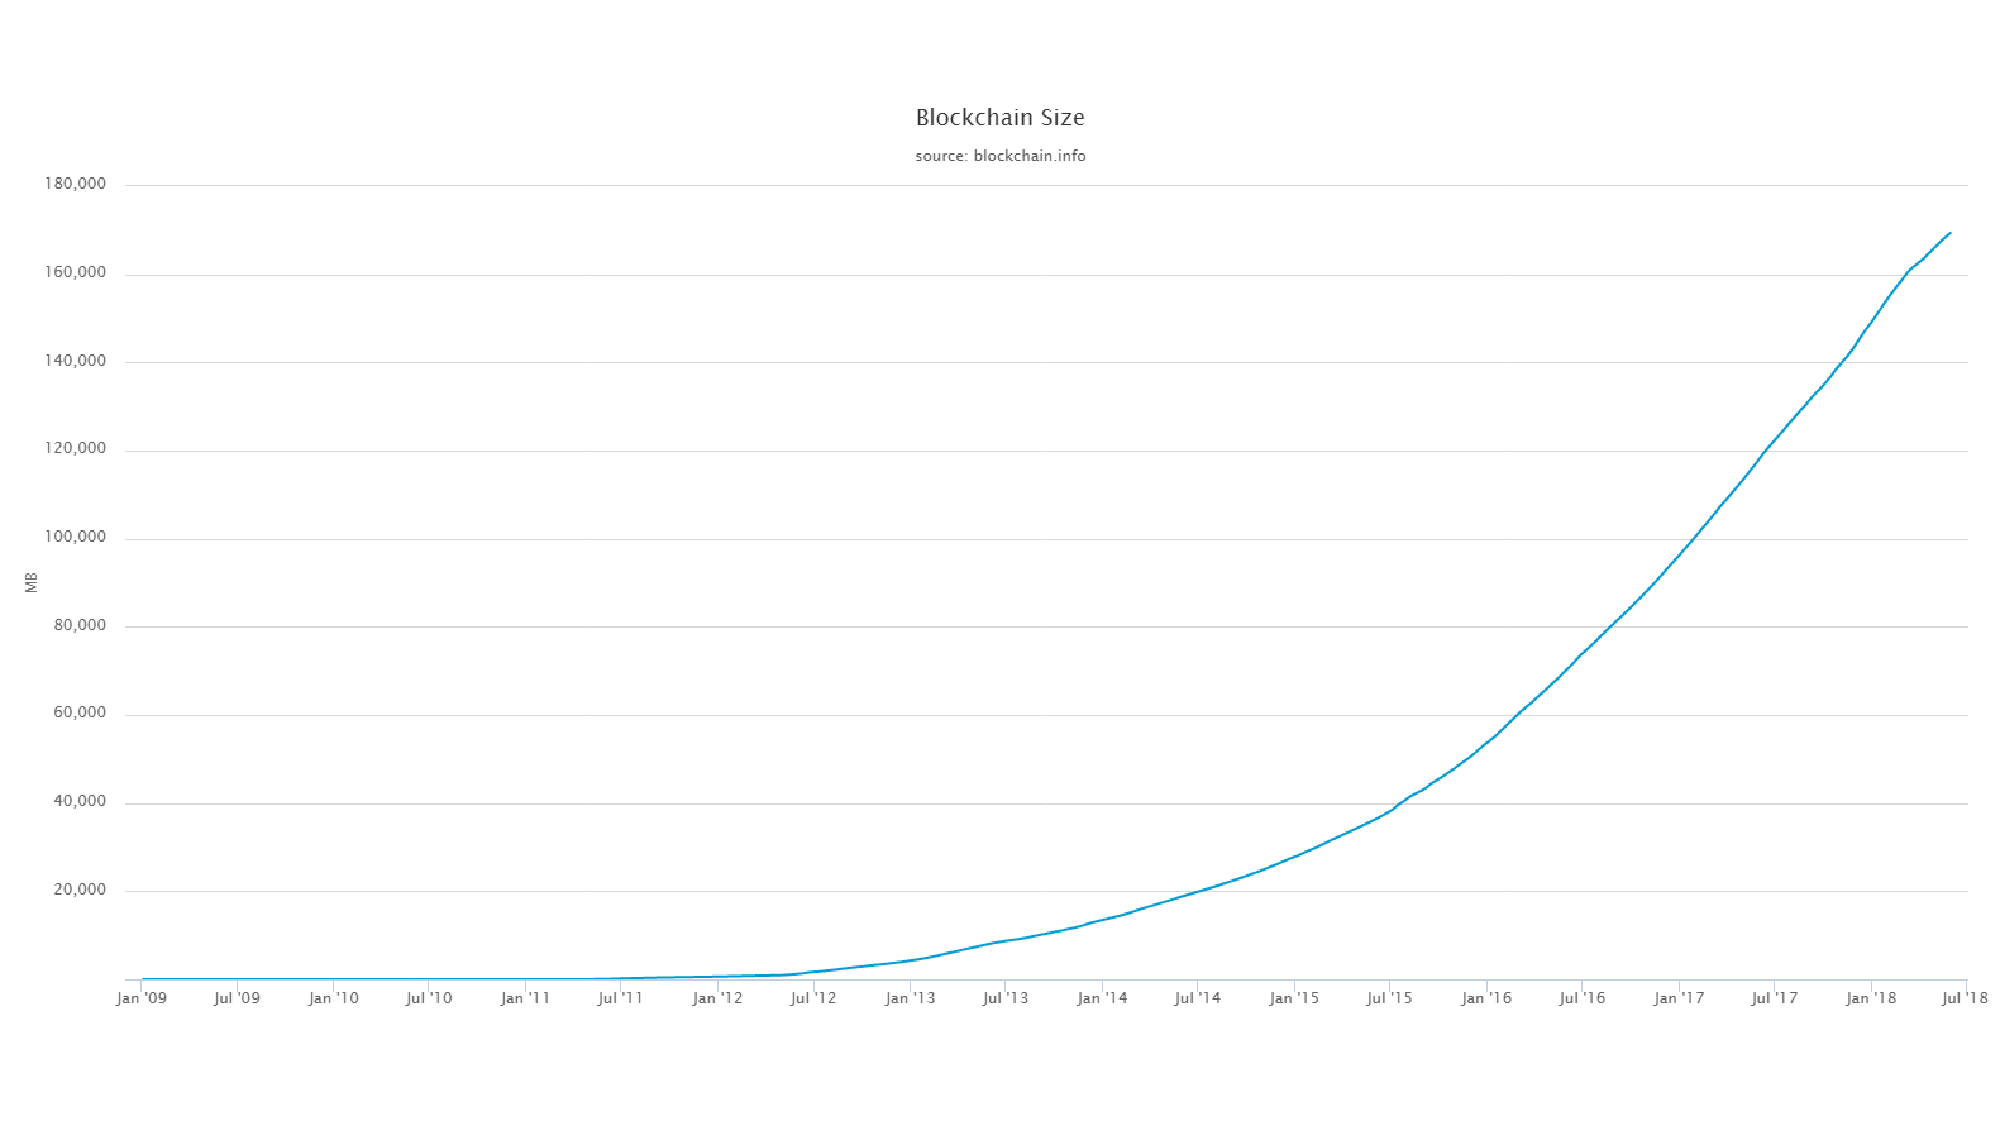
\includepdf[pages=-,nup=1x2]{courses/区块链技术与应用/11-BTC.pdf} 

\subsection{BTC-匿名性}
\subsubsection{匿名与隐私}
Bitcoin and anonymity
匿名和隐私(privacy)保护联系在一起。

比特币中用的化名pseudonymity,比特币的匿名不是真的匿名。匿名性没有现金好,但是现金不容易保管和运输。如果银行用化名,匿名性要比比特币好。区块链的账本是完全公开的,银行的账本不是完全公开的。

不同账户之间关联有可能破坏匿名性。网上购物,允许有多个输入和输出。

Inputs: addr1(4BTC), addr2(5BTC)

Outputs: addr3(6BTC), addr4(3BTC)

addr1和adder2很有可能是同一个人的。输出地址一般有一个找零钱的地址。addr4是找零地址,也可以将输入地址和输出地址关联。常用的比特币钱包就几种。找到其中产生地址的规律就可以关联起来。

地址账户和现实世界的身份产生关联。任何比特币货币和实体世界发生联系,就可能泄漏身份。例如资金的转入和转出、用比特币做支付。商家支持比特币支付,延迟大,交易费贵。

信用卡号码取哈希值公开,但是通过几次特定时间消费,进行过滤后可以定位到人。比特币交易记录都是公开的。

中本聪的匿名性保护的最好,没有花费比特币。

网站Silk road,有人管它叫eBay for illegal drugs。卖的是违禁品,支付用比特币,网络层是TOR,美国用匿名邮寄服务。运行两三年就被查封了。第二版Silk road 2。比特币的匿名性没有我们想象中的那么好。

hide your identity for whom?不想向谁暴露身份?如果是向邻居保持匿名,比较容易实现。

采取什么样的方法尽可能提高匿名性?

application layer

--------

network layer

提高匿名性从两个方面入手。网络层的匿名性比较好解决,普遍的是多路径转发,洋葱路由TOR就是这个原理。应用层把各个不同的币混在一起(coin mixing),让人分不清这些币从哪里来的,真正实施起来有些困难。在区块链里目前没有信誉度高的coin mixing服务,因为它们也要匿名,跑路就没办法了。有一些应用带有coin mixing性质,比如在线钱包,但在线钱包并不保证履行这个功能。加密货币的交易所天然的有coin mixing性质,前提是交易所不会泄漏记录。

保护隐私难度大,本质是区块链账本公开且不可篡改。

\subsubsection{零知识证明}
签名证明知道私钥,但是泄漏了私钥的签名。是不是零知识证明有点争议。

\textbf{同态隐藏}
\begin{itemize}
    \item 加密函数值不会出现碰撞。
    \item 加密函数不可逆。和哈希函数里的hiding property类似。
    \item 同态运算。
\end{itemize}

\includepdf[pages=-,nup=1x2]{courses/区块链技术与应用/12-BTC.pdf} 
\subsection{BTC-比特币引发的思考}
\subsubsection{哈希指针}
\textbf{区块链中的哈希指针怎么传播?}

指针只和本地机器相关。实际系统中用的只有哈希,指针只是一个形式说法。
\begin{figure}[H]
    \centering
    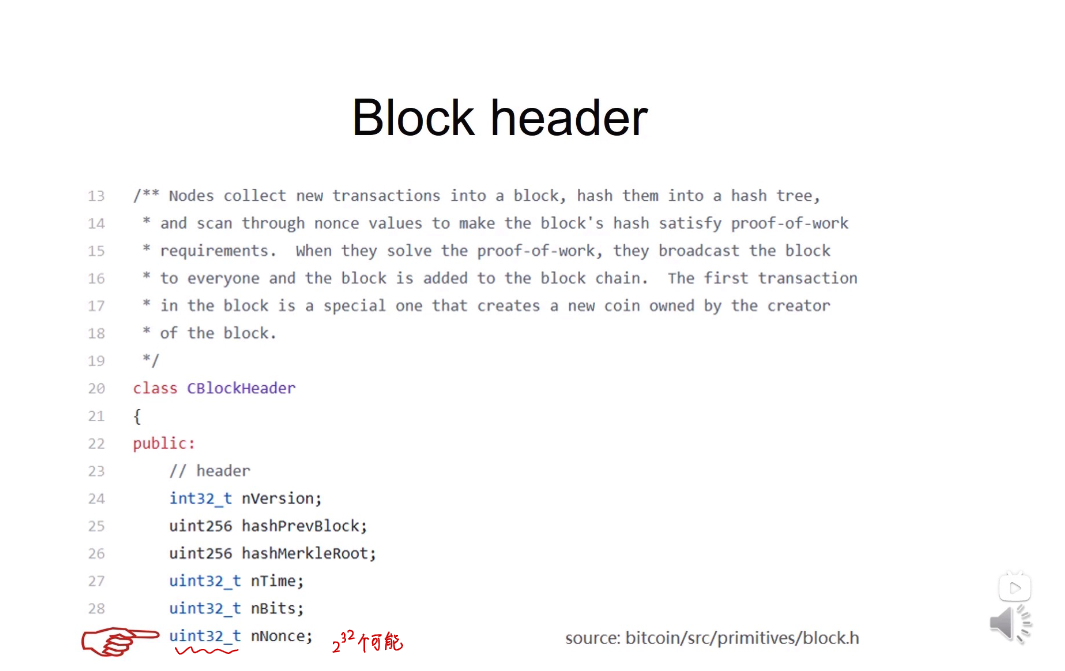
\includegraphics[width=1\textwidth]{courses/区块链技术与应用/lecture13/img1.png} 
\end{figure}
 
\textbf{怎么找到区块内容?}全节点将这些存在(key, value)数据库中,常用的是levelDB数据库。

\subsubsection{区块恋}
截断私钥的做法会降低账户的安全性。比特币中的安全和私钥的长度相关,256位,但是如果截断,只需要猜另一半的私钥就能破解。对多个人的账户,不要用截断私钥的方法,用多重签名MULTISIG。

区块恋中可能会造成死钱,UTXO中的死钱是普遍问题。
\subsubsection{分布式共识}
\textbf{为什么比特币系统能够绕过分布式共识中那些不可能结论?}

严格地说,比特币并没有取得真正意义下的共识。例如分叉。理论和实际有一定距离。

\textbf{远程服务器连不上,如何区分是垮掉还是运行缓慢?}

分布式理论证明在异步(通讯的延迟没有上限)的环境中,不可能区分某台远程服务器是垮掉还是运行缓慢。实际中可以给服务器处人员打电话询问,或者给服务器加一个电话线,可以拨号上网。

\subsubsection{比特币的稀缺性}
挖矿的收益要大于挖矿的开销。比特币早期挖矿难度低,出块奖励多。

总量固定的东西实际不适合作为货币。一个好的货币要有通货膨胀的功能。

\subsubsection{量子计算}
量子计算技术离实用还有很大距离。量子计算对传统金融的冲击更大。

比特币中并没有将账户的公钥直接暴露出来,而是用公钥的哈希。即使用量子计算机,也没办法进行哈希的逆运算。从安全角度来看,比特币中的地址用过一次后就不要再用了。即使是公钥,也不要随便泄漏。

\subsection{ETH-以太坊概述}
以太坊的出块时间变为十几秒。同时改变了mining puzzle,对内存要求高,叫memory hard mining puzzle,限定了ASIC芯片的使用(ASIC resistance)。用权益证明(proof of stake)来替代工作量证明(proof of work)。增加了对智能合约(smart contract)的支持。

BitCoin: decentralized currency, BTC 最小单位Satoshi

Ethereum: decentralized contract, ETH 最小单位Wei

去中心化的货币,可以跨国转账。去中心化的合同,如果合约的签署方来自各国,可以用智能合约。就算是同一个司法管辖权内,司法手段也可能比较麻烦。智能合约的代码一经发布到区块链中,就不可以篡改。

\subsection{ETH-账户}
A $\rightarrow$ B(10BTC),要说明币的来源。B $\rightarrow$ C(3BTC),不说明的话剩下的7个BTC当成gas费了,所以剩下的币要转给自己另外的账户B $\rightarrow$ B‘(7BTC)。

以太坊采用基于账户的模型(account-based ledger)。A $\rightarrow$ B(10ETH),检查交易的合法性只用检查A账户上的钱是否足够,不用说明币的来源。比特币面临的挑战是double spending attack,以太坊天然能防御这一点。

账户的余额不能随便改,因为账户的余额在全节点中维护。

replay attack,重放攻击,A $\rightarrow$ B(10ETH),假设B是恶意的,再把这个交易广播一次,将A的钱扣了两次。比特币中不会出现repaly attack,因为这会导致double spending。以太坊中加一个nonce(实际是一个计数器),记录交易次数,发布交易时加上这个nonce,整个内容由账户进行签名。系统中会维护账户的余额和nonce值。

以太坊中有两类账户,一类是外部账户externally owner account。外部账户状态有balance、nonce(实际是计数器)。通过公私钥对控制。第二类账户是合约账户smart contract account。合约账户不能主动发起一个交易。合约账户有balance、nonce、code、storage。合约账户可以被调用。

以太坊的创始人Vitalik。以太坊支持合约,要求参与者有稳定的身份。用合约实现金融衍生品(financial derivative)。

\subsection{ETH-状态树}
以太坊中将账户地址映射到状态,addr $\rightarrow$ state。地址是160bits,一般表示成40个十六进制的数。

\textbf{以太坊中如何证明某个账户的余额是多少?}

比特币中是对一个区块中的几百到几千个交易构成一个新的Merkle tree。而在以太坊中,如果将所有的账户-状态组织成\textbf{哈希表}结构,将账户组织成Merkle tree,这样需要包括的账户数太多。Merkle tree除了证明某个交易在区块中,还有一个作用是保持全节点中内容的一致性,这也是为什么比特币中要将Merkle tree的根哈希值写在块头里。

如果直接将账户-状态构建成一个\textbf{Merkle tree},问题在于Merkle tree没有提供一个高效的查找和更新的方法。还有一个问题是Merkle tree要不要排序(sorted Merkle tree)?不排序会导致构建Merkle tree是不一样的,算出的根哈希值也不相同。新节点产生是随机的,会插入到Merkle tree中,导致Merkle tree需要更新,可能大半个树需要重构,加入的代价比较大。

\textbf{trie} 字典树,从retrieval中来。分叉数目branching factor。以太坊中是17(加上结束标志位)。trie中地址长度相同,也就是查找长度相同。trie中不会出现碰撞。trie会得到相同的树。更新操作具有局部性,用trie只用访问一个分支。trie的存储会增大。

\textbf{Patricia tree/trie},经过路径压缩的前缀树。如果新插入一个节点,原来压缩的路径可能会展开。插入的节点的键值分布稀疏,压不压缩效果比较大。例如单词misunderstanding、decentralization、disintermediation(去中间商)。

\textbf{MPT(Merkle Patricia tree)},在Patricia tree中把普通指针换成哈希指针。可以计算出根哈希值,写在block header里。根哈希值的作用:防止篡改以及Merkle proof(证明账户余额、证明某个键值不在MPT中)。

以太坊中用的是Modified MPT。合约账户中的存储用的也是MPT。

\textbf{为什么每次改变是新建一个分支而不是直接在原来的MPT中更新数据?}
\begin{figure}[H]
    \centering
    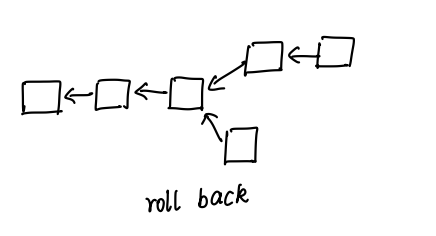
\includegraphics[width=0.4\textwidth]{courses/区块链技术与应用/lecture16/img1.png} 
\end{figure}
比特币中A $\rightarrow$ B(10BTC),回滚比较容易。以太坊中有智能合约,是图灵完备的,以太坊中如果不保存以前的状态,推算出原来的状态是比较难的,要想支持回滚,必须保存历史状态。

以太坊有三棵树:状态树、交易树、收据树。

状态树中保存的是(key,value)。value要经过序列化(RLP,Recursive Length Prefix)再存储。protocol buffer,简称protobuf,作序列化的库。RLP只支持nested array of bytes,字节数组,可以嵌套。

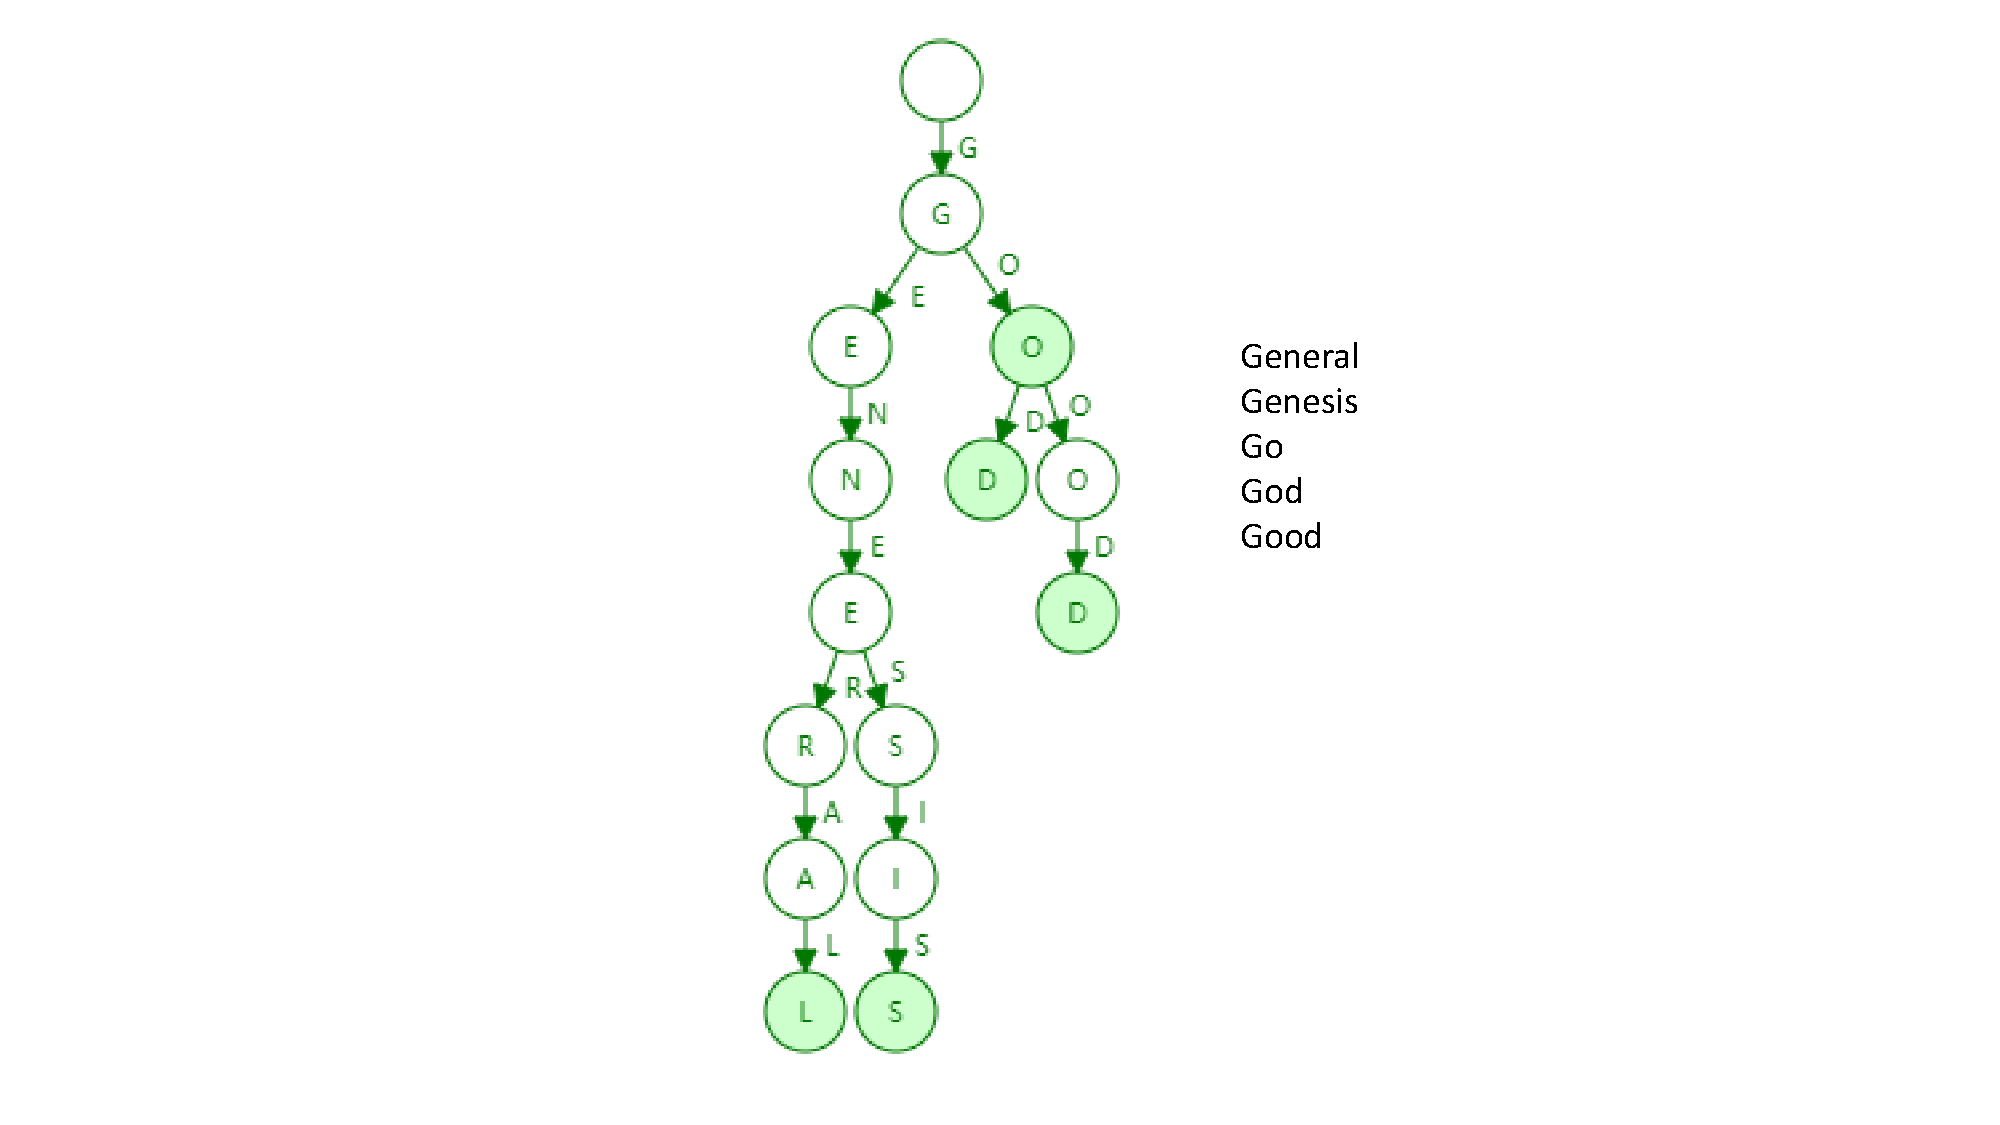
\includepdf[pages=-,nup=1x2]{courses/区块链技术与应用/16-ETH.pdf} 
\section{零知识证明}
\subsection{交互式零知识证明}
参考课程\href{https://zk-learning.org/}{Zero Knowledge Proofs}。
\begin{definition}
	A language $\mathcal{L}$ is a set of binary strings $x$.
\end{definition}
\begin{definition}
	$\mathcal{L}$ is an \textbf{NP}-language (or NP-decision problem), if there is a \textbf{poly$(|x|)$ time} verify $V$ where
	\begin{itemize}
		 \item \textbf{Completeness [True claims have (short) proofs].}
		 
		if $x \in \mathcal{L}$,there is a poly$(|x|)$-long witness $w \in \{0,1\}^*$ s.t. $V(x,w) = 1.$
		\item \textbf{Soundness [False theorems have no proofs].}
		
		if $x \notin \mathcal{L}$, there is no witness. That is, for all $w \in \{0,1\}^*,V(x,w) = 0.$
	\end{itemize}
\end{definition}

\begin{definition}
	$(P, V)$ is an interactive proof for L, if V is probabilistic poly $(|x|)$ time and
	\begin{itemize}
		\item Completeness: If $x \in L$, V always accepts.
		\item Soundness: If $x \notin L$, for all {\color{blue}cheating prover strategy}, V will not accept
		except with negligible probability.
	\end{itemize}
\end{definition}

\begin{definition}
	$(P, V)$ is an interactive proof for L, if V is probabilistic poly $(|x|)$ and
	\begin{itemize}
		\item Completeness: If $x\in L$, $Pr[(P,V)(x)= accept]=1$.
		\item Soundness: If $x \notin L$, for every $P^*$, $Pr[(P^*,V)(x)= accept]=negl(|x|)$
		where $negl(\lambda) \le \frac{1}{polynomial(\lambda)}$ for all polynomial functions.
	\end{itemize}
\end{definition}

\begin{definition}
	$(P, V)$ is an interactive proof for L, if V is probabilistic poly $(|x|)$ and 
	\begin{itemize}
		\item Completeness: If $x\in L$, $Pr[(P,V)(x)= accept] \ge c$
		\item Soundness: If $x \notin L$, for every $P^*$, $Pr[(P^*,V)(x)= accept] \le s$
	\end{itemize}
	Equivalent as long as $ c-s \ge 1/poly(|x|)$.
\end{definition}

\begin{definition}
	class of languages IP =
\{L for which there is an interactive proof\}.
\end{definition}

\begin{definition}
	An Interactive Protocol $(P,V)$ is \textbf{zero-knowledge} for a language L if there exists a PPT algorithm Sim (a simulator) such that for every $x \in L$, the following two probability distributions are poly-time indistinguishable:
	\begin{enumerate}
		\item $view_V(P,V)[x, 1^\lambda]$
		\item $Sim(x, 1^\lambda)$
	\end{enumerate}
\end{definition}
\begin{definition}
	$(P,V)$ is a \textbf{zero-knowledge interactive protocol} if it is complete, sound and zero-knowledge.
\end{definition}

\begin{definition}
	An Interactive Protocol $(P,V)$ is zero-knowledge for a language L if for every PPT $V^*$, there exists a poly time simulator Sim s.t. for every $x \in L$,
	$$
	view_V(P,V)[x] \approx Sim(x,1^\lambda)
	$$
\end{definition}

\textbf{Flavors of Zero Knowledge}
\begin{itemize}
	\item Computationally indistinguishable distributions = CZK
	\item Perfectly identical distributions = PZK
	\item Statistically close distributions = SZK
\end{itemize}

Consider $L_R=\{x: \exists w \text{ s.t. }  R(x,w)= accept \}$ for poly-time relation $R$.
\begin{definition}
	$(P,V)$ is a \textbf{proof of knowledge} (POK) for $L_R$ if :
	$\exists$ PPT (knowledge) extractor algorithm E s. t. $\forall x$ in L,
	in expected poly-time $E^P(x)$ outputs w s.t. R(x,w)=accept. {\color{blue}[if $Prob[(P,V)(x)=accept] > \alpha$, then $E^P(x)$ runs in expected poly$(|x|,1/ \alpha)$ time]}
\end{definition}

\begin{theorem}[GMW86,Naor]
	If one-way functions exist, then every L in NP has \textbf{computational zero knowledge interactive proofs}.
\end{theorem}

Properties of a Bit Commitment Protocol (Commit, Decommit) between Sender S and Receiver R
\begin{itemize}
	\item \textbf{Hiding}: $\forall$ receiver $R^*$ , after {\color{blue} commit} stage $\forall b, b' \in {0,1}$, view of sender $R^*$ $\{ View_{R^*}(Sender(b),R^*)(1^k)\}$ $ \approx_c  \{ View_{R^*}(Sender(b'),R^*)(1^k)\}$ [k = sec.param]
	\item \textbf{Binding}: $\forall$ sender $S^*$, after {\color{blue} commit} and {\color{blue} decommit stage}, Prob[R will accept two different values b and b’] < negl(k), K-security parameter
\end{itemize}

\textbf{Protocol design applications}

Generally: A tool to enforce honest behavior {\color{violet}in protocols} without revealing any information. Idea: protocol players sends along with each next-msg, a ZK proof that next-msg= Protocol(history h, randomness r) on history h and c=commit(r) Possible since {\color{violet}$L=\{\exists r \text{ s.t. next-msg = Protocol}(h.r) \text{ and } c = commit(r)\}$} in NP.

\textbf{Arthur-Merlin Games [BaM85]}
\begin{theorem}[GoldwasserSipser86]
	AM (protocols with Public Coins) = IP
\end{theorem}
AM Protocols enable "in practice" removal of interaction: the Fiat-Shamir Paradigm[FS87].
Fiat-Shamir Heuristic:
If H is random-oracle, then completeness and soundness hold.

Warning: this does \textbf{NOT} mean every interactive ZK proof can transform to AM
protocols and then use Fiat-Shamir heuristic, since IP = AM transformation requires extra super-polynomial powers from Merlin. And for Fiat-Shamir heuristic to work, Prover must be computationally bounded so not to be able to invert H. Yet, many specific protocols, can benefit from this heuristic.

\subsection{Modern SNARKs}
参考\href{https://www.youtube.com/watch?v=bGEXYpt3sj0}{ZKP MOOC Lecture 2: Overview of Modern SNARK Constructions}。

\subsubsection{arithmetic circuits}
对于一些素数$p \ge 2$,选定一个有限域$\mathbb{F} = \{0, \cdots, p-1\}$。算术电路:$C: \mathbb{F}^n \rightarrow \mathbb{F}$
\begin{itemize}
	\item 一个有向无环图,其中用$1,x_1,\cdots,x_n$作为输入,内部节点之间有$+,-,\times$运算。
	\item 算术电路定义了一个$n$变量的多项式的估计。
\end{itemize}
记$|C| =$ \#gates in $C$,就是电路门数目。
\begin{figure}[H]
    \centering
    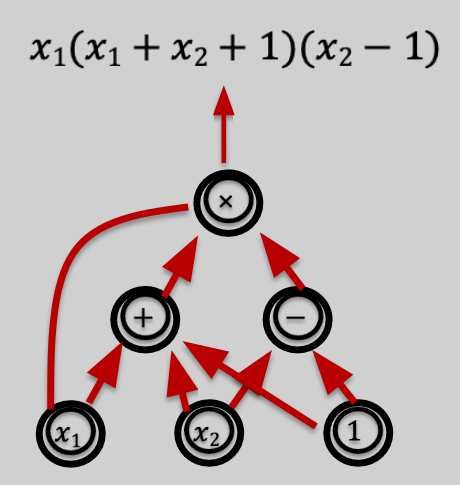
\includegraphics[width=0.4\textwidth]{./img/arithmetic_circuit.png} 
\end{figure}
文章\href{https://secbit.io/blog/2019/07/31/zero-knowledge-and-proof/}{初识「零知识」与「证明」}中说明了可验证计算与电路可满足性问题。所谓的\textbf{电路可满足性}就是指,存在满足电路的一个解。如果这个解的输出值等于一个确定值,那么这个解就能「表示」电路的计算过程。\textbf{零知识的电路可满足性证明协议}提供了一种最直接的保护隐私/敏感数据的技术。

\textbf{Structured vs. unstructured circuits}

An unstructured circuit: a circuit with aribitary wires.

A structured circuit:
\begin{figure}[H]
    \centering
    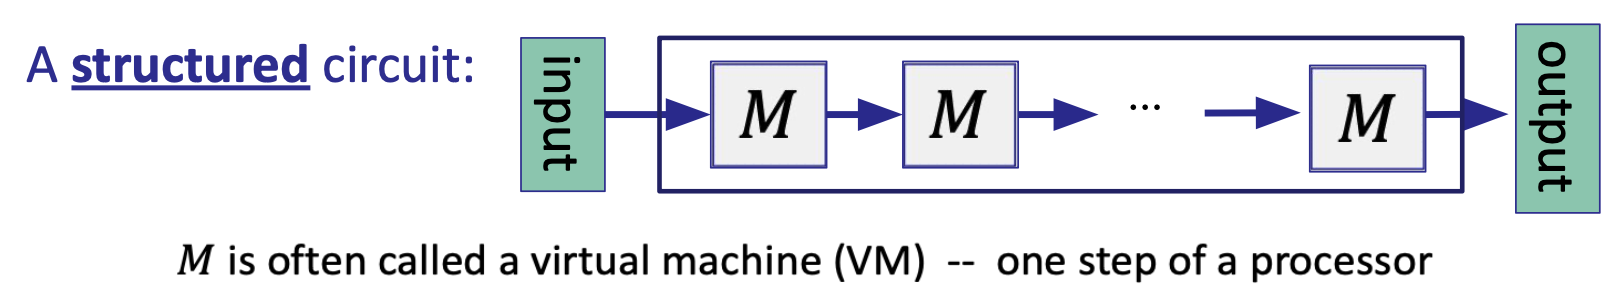
\includegraphics[width=0.9\textwidth]{./img/structured_circuit.png} 
\end{figure}

\subsubsection{NARK}
NARK: Non-interactive ARgument of Knowledge

对于公开的算术电路:$C(x,w) \rightarrow \mathbb{F}$,其中$x$是$\mathbb{F}$中公开的陈述(statement),$w$是$\mathbb{F}^m$中的秘密(secret witness)。预处理过程(setup)是:$S(c) \rightarrow (pp,vp)$。
\begin{figure}[H]
    \centering
    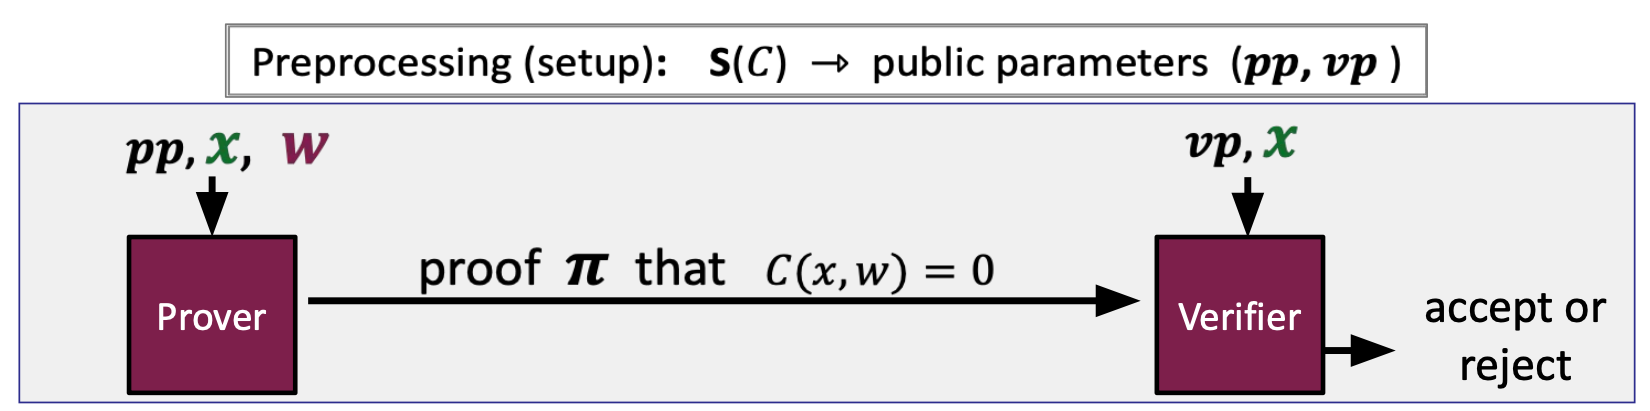
\includegraphics[width=0.9\textwidth]{./img/preprocessing.png} 
\end{figure}
一个预处理的NARK是一个三元组$(S,P,V)$:
\begin{itemize}
	\item $S(C) \rightarrow$ prover和verifier的公开参数$(pp,vp)$
	\item $P(pp,x,w) \rightarrow$ 证明 $\pi$
	\item $V(vp,x,\pi) \rightarrow$ 接受或拒绝
\end{itemize}

NARK中要求:
\begin{itemize}
	\item \textbf{Complete}: $\forall x,w: C(x,w) = 0 \Rightarrow Pr[V(vp,x,P(pp,x,w))=accept] =1$
	\item Adaptively \textbf{knowledge sound}: V accepts $\Rightarrow$ P "knows" $w$ s.t. $C(x,w)=0$ (存在一个知识提取器能从$P$中提取出有效的$w$)
	\item 可选: \textbf{Zero knowledge}: $(C,pp,vp,x,\pi)$没有泄漏任何关于$w$的新的知识
\end{itemize}

\subsubsection*{A succinct preprocessing NARK}
\begin{figure}[H]
    \centering
    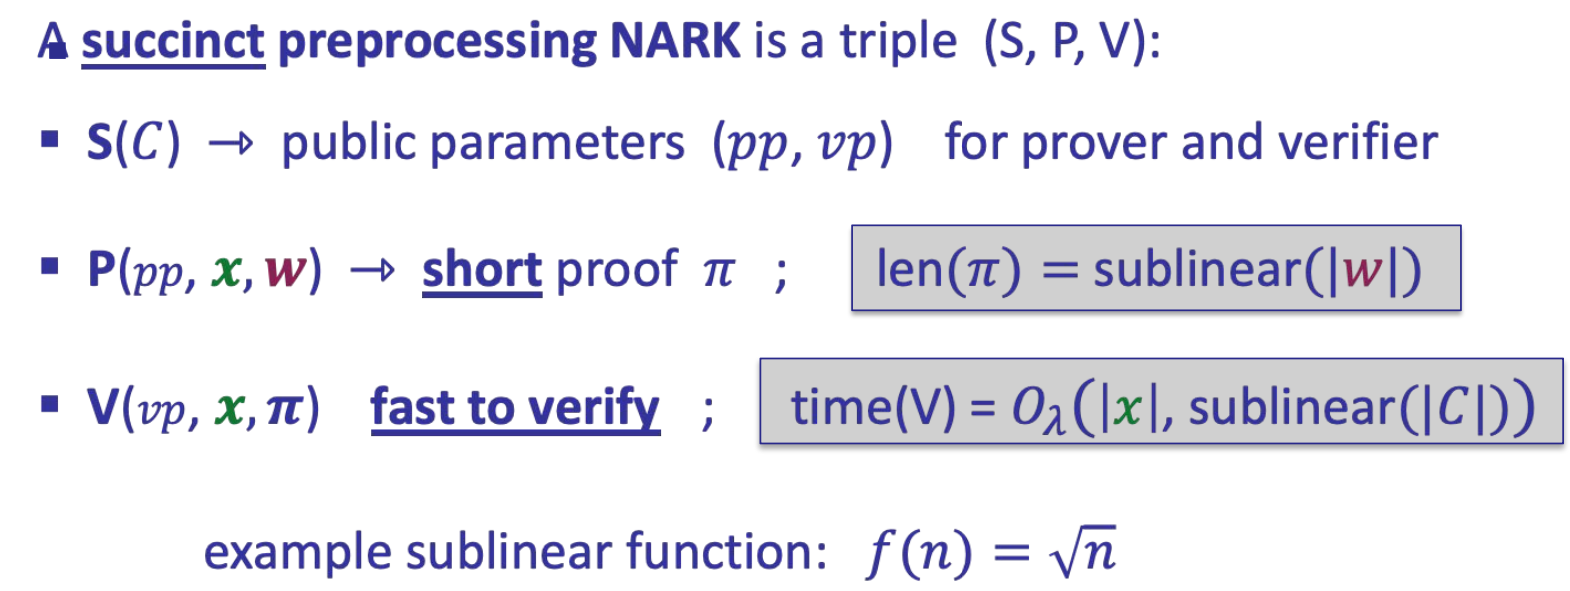
\includegraphics[width=0.9\textwidth]{./img/a_succinct_NARK.png} 
\end{figure}

\subsubsection*{A strongly succinct preprocessing NARK}
\begin{figure}[H]
    \centering
    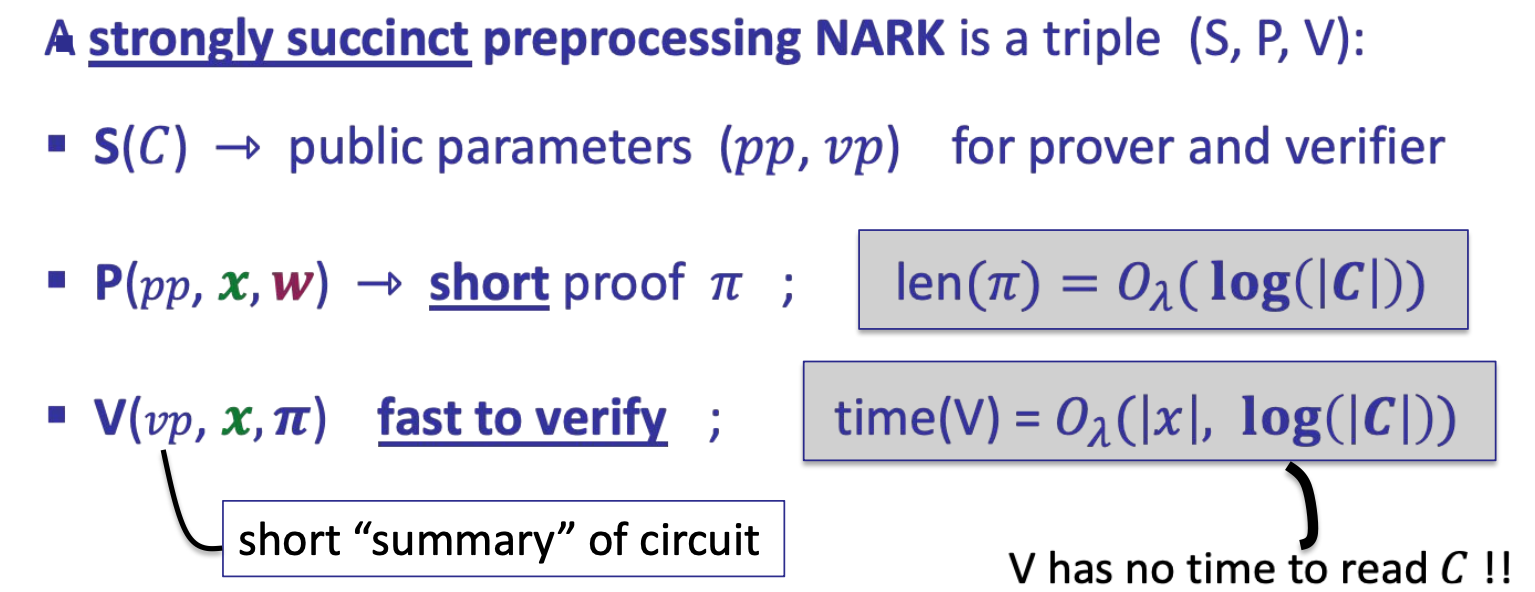
\includegraphics[width=1\textwidth]{./img/a_strongly_succinct_NARK.png} 
\end{figure}
SNARK: 就是一个NARK(complete and knowledge sound)是succint.

zk-SNARK: 就是一个SNARK是zero knowledge.

\subsubsection*{Types of preprocessing Setup}
\begin{figure}[H]
    \centering
    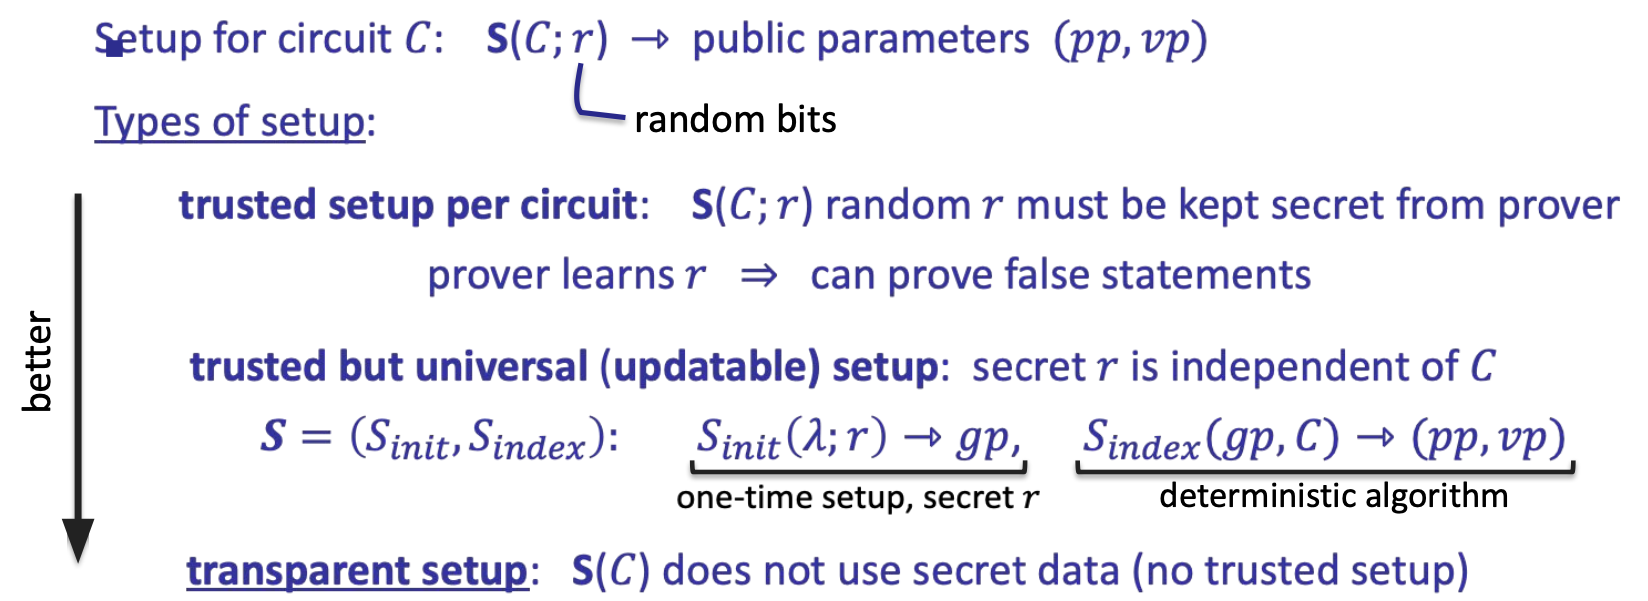
\includegraphics[width=1\textwidth]{./img/types_of_preprocessing_setup.png} 
\end{figure}

\subsubsection*{knowledge soundness}

\begin{figure}[H]
    \centering
    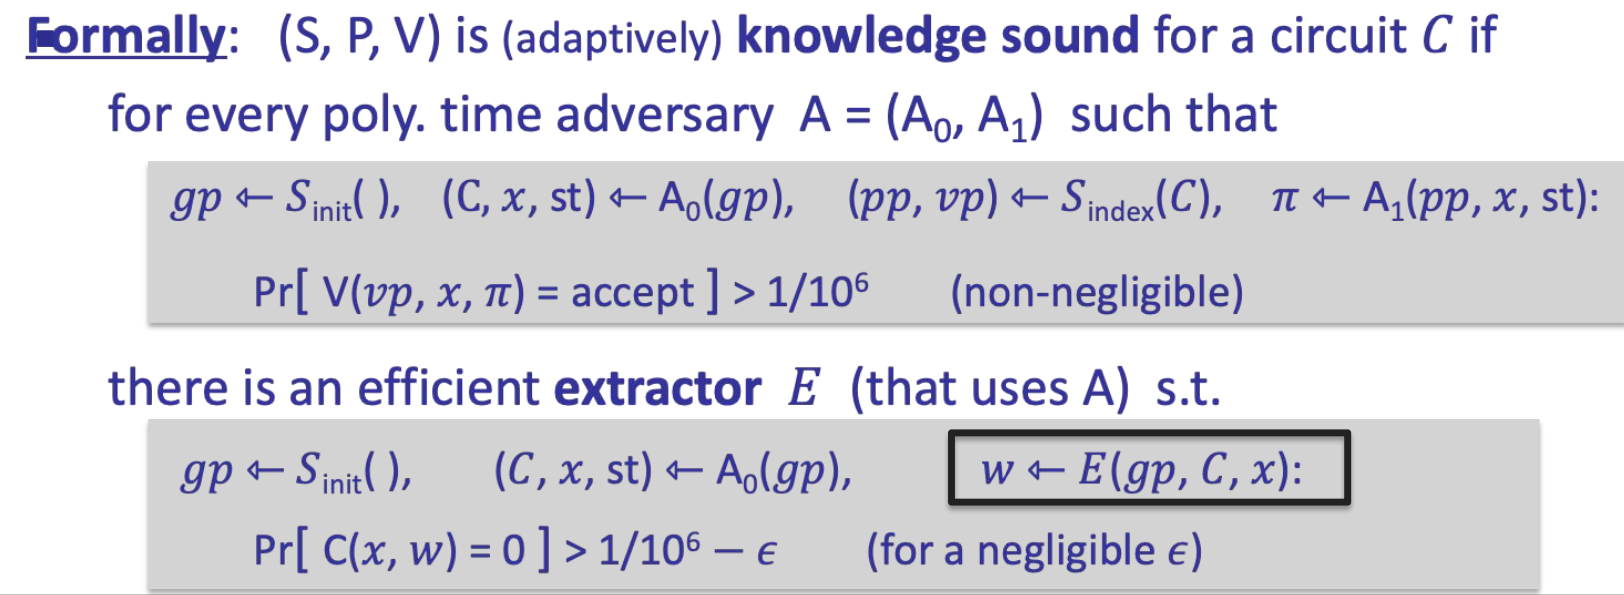
\includegraphics[width=1\textwidth]{./img/knowledge_soundness.png} 
\end{figure}

\subsubsection{Building an efficient SNARK}

\section{Circom}
参考课程\href{https://zkiap.com/}{[MIT IAP 2023] Modern Zero Knowledge Cryptography}、\href{https://zkshanghai.xyz/}{ZK Shanghai 2023}。Circom 2文档见\href{https://docs.circom.io/circom-language/signals/}{这里}。

\subsection{Signals}
signal可用input、output标识,或者不标识表示中间的singal。
\begin{lstlisting}
signal input in;
signal output out[N];
signal inter;
\end{lstlisting}
单个的singal始终是私有的。如果有input标识,input可以在main中明确公开,如果没明确说明也是私有的。singal output是公开的(不能成为私有的)。
\begin{lstlisting}
pragma circom 2.0.0;

template Multiplier2(){
   //Declaration of signals
   signal input in1;
   signal input in2;
   signal output out;
   out <== in1 * in2;
}

component main {public [in1,in2]} = Multiplier2();
\end{lstlisting}

从程序员的角度来看,在电路外面只能看到public input和output,因此不能获取到中间的signal。

\textbf{signal是不可变的},一旦给signal指定了一个值,就不能再改变了。在编译的时候,始终将singal认为是未知的(Unknowns)。这么做的原因是在一开始就明确结构,而不是依赖于编译器是否具有能检测出这些singal是否始终保持不变的能力。
\begin{lstlisting}
pragma circom 2.0.0;

template A(){
   signal input in;
   signal output outA; 
   var i = 0; var out = 0;
   while (i < in){
      out++; i++;
   }
   outA <== out;
}

template B(){
   component a = A();
   a.in <== 3;
}

component main = B();
\end{lstlisting}
上面这个例子有一个编译错误,因为signal \verb|outA|取决于signal \verb|in|,尽管是一个常数3。

给signal指定值可以用\verb|<--|、\verb|<==|、\verb|-->|或者\verb|==>|。\verb|<==|和\verb|==>|是安全的操作,因为在指定值的同时也生成约束。使用\verb|<--|和\verb|-->|一般是危险的,应该只在指定的表达式不能包含在约束中的情况下使用,例如:
\begin{lstlisting}
out[k] <-- (in >> k) & 1;
\end{lstlisting}

变量是可变的,前面的关键词是\verb|var|。
\begin{lstlisting}
var x;
\end{lstlisting}
变量的指定用符号\verb|=|。指定是一个statement,并且不返回任何值,因此不能作为表达式的一部分,这会避免\verb|=|的错误使用。任何表达式中包含\verb|=|都会导致编译错误。下面的两个例子会导致编译错误。

\begin{lstlisting}
a = (b = 3) + 2;
\end{lstlisting}
\begin{lstlisting}
var x;
if (x = 3) {
	var y = 0;
}
\end{lstlisting}

\subsection{Templates}
\subsubsection{Templates \& Components}
\subsubsection*{Templates}
Templates不能包含局部函数或者template函数。在定义输入信号的同一template中为输入信号分配值也会导致错误“Exception caused by invalid assignment”,例如:
\begin{lstlisting}
pragma circom 2.0.0;

template wrong (N) {
   signal input a;
   signal output b;
   a <== N;
}

component main = wrong(1);	
\end{lstlisting}
因为对于输入信号来说,本来就会有输入值,如果再赋值,就会导致错误。

template的实例用关键词\verb|component|,并且提供必要的参数。参数的值需要再编译时就是已知的常数。
\begin{lstlisting}
component c = tempid(v1,...,vn);
\end{lstlisting}
下面这个例子会报错“Every component instantiation must be resolved during the constraint generation phase”。
\begin{lstlisting}
pragma circom 2.0.0;

template A(N1,N2){
   signal input in;
   signal output out; 
   out <== N1 * in * N2;
}


template wrong (N) {
   signal input a;
   signal output b;
   component c = A(a,N); 
}

component main {public [a]} = wrong(1);
\end{lstlisting}
\subsubsection*{Components}
一个component定义了一个算术电路,接收N个输入信号,产生M个输出信号和K个中间信号。为了得到一个component的输入或输出信号,用\textbf{点}记号。在component外部其他的信号是不可见的。
\begin{lstlisting}
c.a <== y*z-1;
var x;
x = c.b;
\end{lstlisting}
component实例化只有在其所有输入信号都被分配给具体的值后才会被触发。component的输出信号只有在所有输入都设置时才能使用,否则会产生编译错误,例如:
\begin{lstlisting}
	pragma circom 2.0.0;

	template Internal() {
	   signal input in[2];
	   signal output out;
	   out <== in[0]*in[1];
	}
	
	template Main() {
	   signal input in[2];
	   signal output out;
	   component c = Internal ();
	   c.in[0] <== in[0];
	   c.out ==> out;  // c.in[1] is not assigned yet
	   c.in[1] <== in[1];  // this line should be placed before calling 
	   // c.out
	}
	
	component main = Main();
\end{lstlisting}
component像信号一样是不可变的。一个component可以先声明再定义。如果有好几处初始化的地方,那么它们需要是同一个template的实例。
\begin{lstlisting}
template A(N){
   signal input in;
   signal output out;
   out <== in;
}

template C(N){
   signal output out;
   out <== N;
}
template B(N){
  signal output out;
  component a;
  if(N > 0){
     a = A(N);
  }
  else{
     a = A(0);
  }
}

component main = B(1);
\end{lstlisting}
如果\verb|a = A(0);|改为\verb|a = C(0);|,就会报错“Assignee and assigned types do not match”.

可以定义component数组,但是初始化要一个一个进行,同样地,所有的在同一个数组中的component必须是相同的template的实例。例如:
\begin{lstlisting}
template MultiAND(n) {
	signal input in[n];
	signal output out;
	component and;
	component ands[2];
	var i;
	if (n==1) {
		out <== in[0];
	} else if (n==2) {
			and = AND();
		and.a <== in[0];
		and.b <== in[1];
		out <== and.out;
	} else {
		and = AND();
	var n1 = n\2;
		var n2 = n-n\2;
		ands[0] = MultiAND(n1);
		ands[1] = MultiAND(n2);
		for (i=0; i<n1; i++) ands[0].in[i] <== in[i];
		for (i=0; i<n2; i++) ands[1].in[i] <== in[n1+i];
		and.a <== ands[0].out;
		and.b <== ands[1].out;
		out <== and.out;
	}
}
\end{lstlisting}
如果component中是独立的,也就是输入不依赖于其他的输出,那么这些部分的计算可以在parallel中完成,加上标签\verb|parallel|. 
\begin{lstlisting}
template parallel NameTemplate(...){...}
\end{lstlisting}
如果用了这个标签,得到的C++文件会包含并行代买来计算witness。注意,这种并行性只能在C++ witness生成器中使用。

\subsubsection{Pragma}
\subsubsection*{Version Pragma}
所有后缀为\verb|.circom|的文件都需要以一个\verb|pragma|指引开始,说明编译器的版本。
\begin{lstlisting}
pragma circom xx.yy.zz;
\end{lstlisting}
如果没有说明,会默认最新版本并抛出一个警告。
\subsubsection{Functions}
\subsection{基本操作}
\subsubsection{Field Elements}
电路里的值是域Z/pZ里的值,其中素数p是提前设定好的:
\begin{lstlisting}
p = 21888242871839275222246405745257275088548364400416034343698204186575808495617.
\end{lstlisting}
因此,电路里的元素都是在模p下的算术操作。
\subsubsection{条件表达式}

\subsection{条件约束}

\section{Groth16}
\section{文章}
\subsection{椭圆曲线}
\subsubsection{A (Relatively Easy To Understand) Primer on Elliptic Curve Cryptography}
文章见\href{https://blog.cloudflare.com/a-relatively-easy-to-understand-primer-on-elliptic-curve-cryptography/}{这里}.
\subsection{zk-SNARKs}
\subsubsection{Exploring Elliptic Curve Pairings}
文章见\href{https://medium.com/@VitalikButerin/exploring-elliptic-curve-pairings-c73c1864e627}{这里}.

椭圆曲线加密涉及数学上说的“点”(也就是有$(x,y)$坐标的二维点),这些“点”可以进行加法和减法运算(例如计算$R=P+Q$的坐标,也可以用一个整数去乘以一个点,例如$P * n = P + P + \cdots + P$)。
\begin{figure}[H]
    \centering
    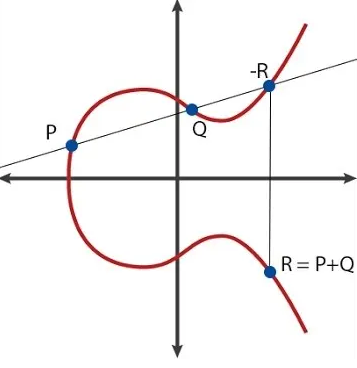
\includegraphics[width=0.5\textwidth]{./img/ExploringEllipticCurvePairings/EllipticCurve.png} 
\end{figure}
存在一个特殊的点叫做“无穷远点”($O$),在点运算中等价于零,$P + O = P$.同样,一个曲线也有一个“阶”,即对于任意点$P$,存在一个数$n$,使得$P * n = O$.“生成点”$G$,可以理解为数字$1$。理论上,一个曲线上任意点(除了点$O$)都可以是$G$。

$e(P,Q)$就是双线性映射,双线性意味着满足如下约束:
$$
e(P,Q+R)=e(P,Q) * e(P,R) 
$$
$$
e(P+S,Q) = e(P,Q) * e(S,Q)
$$

素数域包含数字$0,1,2,\cdots p-1$,$p$是一个素数,可以进行如下运算:
\begin{lstlisting}
  a + b:  (a + b) % p
  a * b:  (a * b) % p
  a - b:  (a - b) % p
  a / b:  (a * b^(p-2)) % p
\end{lstlisting}
这里除法比较特殊,因为我们希望$a/b$之后还是整数,也就是找到$x * b = a \mod p$,根据费马小定理,$b^{p-1} = 1 \mod p$,因此$x = a * b^{p-2} \mod p$.

\textbf{扩张或扩域(extension field)}。一个常见的扩域的例子就是是实数域到复数的扩张,在实数域上添加一个元素$\sqrt{-1}=i$.基本上,扩张需要在一个存在的域上进行,然后床照一个新的元素,定义这个元素和原来存在元素之间关系($i^2 + 1 = 0$),确保这个方程不会对原来域中的任意数都成立。
\begin{figure}[H]
	\centering
	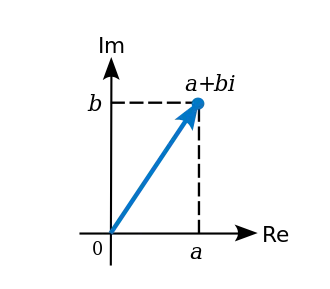
\includegraphics[width=0.6\textwidth]{img/ExploringEllipticCurvePairings/extension_field.png}
\end{figure}
也可以在素数域上进行扩张,例如在素数域模7上用上面提到的$i$进行扩张,可以这样做:
\begin{lstlisting}
  (2 + 3i) + (4 + 2i) = 6 + 5i
  (5 + 2i) + 3 = 1 + 2i
  (6 + 2i) * 2 = 5 + 4i
  4i * (2 + i) = 3 + i
\end{lstlisting}
对于最后一个$4i * (2 + i)$,由于有模7操作,因此$4i * (2 + i) = 8i - 4 = i + 3$. 除法:
\begin{lstlisting}
  a / b:  (a * b^(p^2-2)) % p
\end{lstlisting}
注意这里的费马小定理中用$p^2$替换了$p$。更高效的计算方法可以使用Extended Euclidean Algorithm. 对于域中的任意$x$有$x^{p^2-1}=1$,所以称$p^2-1$为域中multiplicative group的阶。

对于实数,\href{https://en.wikipedia.org/wiki/Fundamental_theorem_of_algebra}{代数基本定理}保证了二次扩张(也就是复数)是完备的,不能再继续扩张了,因为一些新的元素$j$和存在的复数的任何数学关系,可能结果至少是一个已经满足关系的复数。在素数域上不存在这个问题,可以进行三次扩张(其中数学关系是一些新的元素$w$和存在的域元素,$1$,$w$,$w^2$之间是相互线性独立的),更高阶的扩张也是类似的。

一个椭圆曲线对是一个映射$G2 \times G1 \rightarrow Gt$,其中
\begin{itemize}
	\item d
\end{itemize}

\section{Semaphore}
\subsection{快速上手}
官方文档见\href{https://semaphore.appliedzkp.org/}{这里}。

Semaphore是一个零知识协议,允许作为可证明的组成员发出信号,而无需透露身份。此外,它提供了一种简单的机制来防止双重信号。用例包括私人投票、举报、匿名 DAOs 和混合器。

快速安装步骤见\href{https://semaphore.appliedzkp.org/docs/quick-setup}{这里}。
\subsection{Guides}
\subsubsection{Identitiies}
为了加入一个 Semaphore 组,用户必须首先创建一个 Semaphore 身份。 信号量标识包含两个随标识生成的值:
\begin{itemize}
	\item Identity trapdoor
	\item Identity nullifier
\end{itemize}
为了使用和验证身份,身份拥有者必须这道trapdoor和nullifier的值。为了防止伪造,拥有者必须保持这两个值为私有的。

使用\verb|@semaphore-protocol/identity|库创建一个Semaphore身份。

\end{document}